%%%%%
%%
%% Sample document ``thesis.tex''
%%
%% Version: v0.2
%% Authors: Jean Martina, Rok Strnisa, Matej Urbas
%% Date: 30/07/2008
%%
%% Copyright (c) 2008-2011, Rok Strniša, Jean Martina, Matej Urbas
%% License: Simplified BSD License
%% License file: ./License
%% Original License URL: http://www.freebsd.org/copyright/freebsd-license.html
%%%%%

% Available documentclass options:
%
%   <all `report` document class options, e.g.: `a5paper`>
%   withindex   - enables the index. New index entries can be added through `\index{my entry}`
%   glossary    - enables the glossary.
%   techreport  - typesets the thesis in the technical report format. firstyr     - formats the document as a first-year report. times       - uses the `Times` font. backrefs    - add back references in the Bibliography section
% For more info see `README.md`
\documentclass[withindex,glossary,openany]{cam-thesis}

% Citations using numbers
\usepackage[numbers]{natbib}

\usepackage{fancyhdr}

\usepackage{lastpage}       % ``n of m'' page numbering
\usepackage{lscape}         % Makes landscape easier

\usepackage{verbatim}       % Verbatim blocks
\usepackage{listings}       % Source code listings
\usepackage{epsfig}         % Embed encapsulated postscript
\usepackage{array}          % Array environment
\usepackage{array}          % Array environment
\usepackage{enumitem}       % Required by Tom Johnson's exam question header

\usepackage{hhline}         % Horizontal lines in tables
\usepackage{siunitx}        % Correct spacing of units
\usepackage{amsmath}        % American Mathematical Society
\usepackage{amssymb}        % Maths symbols
\usepackage{amsthm}         % Theorems

\usepackage{ifthen}         % Conditional processing in tex
\usepackage{tabularx}

\usepackage[skip=0.5cm]{parskip}

\usepackage[top=3cm,
            bottom=3cm,
            inner=2cm,
            outer=2cm]{geometry}

% If you have any additional \usepackage commands, or other
% macros or directives, put them here.  Remember not to edit
% files in the template directory because any changes will
% be overwritten when template updates are issued.
\usepackage{float,graphicx}
\usepackage{amsmath}
\usepackage{amssymb}
\usepackage{caption}
\usepackage{subcaption}
\usepackage{wrapfig}
\usepackage{listings}

\lstset{
	basicstyle=\ttfamily,
	literate={~} {$\sim$}{1}
}

\usepackage[absolute,overlay]{textpos}

\newcolumntype{C}{>$c<$}
\graphicspath{ {./images/} }

\newcommand{\notimplies}{%
  \mathrel{{\ooalign{\hidewidth$\not\phantom{=}$\hidewidth\cr$\implies$}}}}
\newcommand{\Mod}[1]{\ (\mathrm{mod}\ #1)}
\newcommand{\Z}{\mathbb{Z}}
\newcommand{\R}{\mathbb{R}}
\newcommand{\Q}{\mathbb{Q}}
\newcommand{\N}{\mathbb{N}}

%%%%%%%%%%%%%%%%%%%%%%%%%%%%%%%%%%%%%%%%%%%%%%%%%%%%%%%%%%%%%%%%%%%%%%%%%%%%%%%%
%% Thesis meta-information
%%


\pagenumbering{gobble}
%% The title of the thesis:
\title{Delay-Tolerant Link-State Routing}

%% The full name of the author (e.g.: James Smith):
\author{Ben Andrew}

%% College affiliation:
\college{Magdalene College}

%% College shield [optional]:
\collegeshield{CollegeShields/Magdalene}

%% Submission date [optional]:
% \submissiondate{November, 2042}

%% You can redefine the submission notice [optional]:
\submissionnotice{This dissertation is submitted for Part II of the Computer Science Tripos in 2022}

%% Declaration date:
\date{May, 2022}

%% PDF meta-info:
\subjectline{Computer Science}

%%%%%%%%%%%%%%%%%%%%%%%%%%%%%%%%%%%%%%%%%%%%%%%%%%%%%%%%%%%%%%%%%%%%%%%%%%%%%%%%
%% Contents:
%%
\begin{document}

%%%%%%%%%%%%%%%%%%%%%%%%%%%%%%%%%%%%%%%%%%%%%%%%%%%%%%%%%%%%%%%%%%%%%%%%%%%%%%%%
%% Title page, abstract, declaration etc.:
%% -    the title page (is automatically omitted in the technical report mode).
\frontmatter{}

%%%%%%%%%%%%%%%%%%%%%%%%%%%%%%%%%%%%%%%%%%%%%%%%%%%%%%%%%%%%%%%%%%%%%%%%%%%%%%%%
%% Dissertation body:
%%

%%%%%%%%%%%%%%%%%%%%%%%%%%%%%%%%%%%%%%%%%%%%%%%%%%%%%%%%%%%%%%%%%%%%%%%%%%%%%%%%
%% Introduction
%%

%The project contains 4605 lines of code, consisting of 3944 lines of C and 661 lines of Python

\pagebreak

\chapter{Introduction}

\pagenumbering{arabic}

% JCW: Weak intro.  Start with why, e.g. "Despite the best efforts of network engineers, achieving the reliability required to support traditional routing protocols is impractical in many situations"

Despite the best efforts of network engineers, achieving reliable communications using traditional routing protocols is inefficient and impractical in many situations. In environments with low network-level reliability such as remote or developing regions, protocols like OSPF can have large packet drop rates, or even provide no end-to-end communication whatsoever. The retransmission costs required to fix this can place strain on already limited resources.

This project aims to evaluate delay-tolerant modifications made to a link-state routing protocol for network environments with low reliability. It is motivated by similar conditions being seen in network infrastructure in remote developing regions, where issues such as unreliable power can cause severe and unpredictable drops in packet delivery. We see how modifications made to the routing protocol can reduce this.

% JCW --- this needs to be much longer.  I want more motivation in here --- why should I care about this?

% IMO a structure like this would help:

% 1 paragraph about why we should care about faulty networks
% 1 paragraph about why we need routing protocols for faulty networks
% 1 paragrapha bout how OSPF attempts to address this problem (and where if falls apart)
% 1 paragraph about how DTLSR attempts to address this problem
% 1 paragraph about what you implemented
% 1 paragraph summarising the reuslts of your evaluation -- does that make sense?

\section{Background and Motivation}

%JCW --should be more active -- s/one problem.../routing packets from one note to anohter on ... is challenging.
A challenging problem in networking is that of routing packets from one side of the network to another, on a path hopping from node to node. A routing protocol describes how routers communicate with each other to distribute information about the topology of the network, in order for each router to choose optimal paths to other nodes, and thus make optimal local forwarding decisions for incoming packets. Link-state protocols are one of the two main classes of routing protocols, and aim for every router in the network to have a full view of the network topology. When a change occurs in the network that information is propagated outwards from router to router, with the change being incorporated into each router's internal representation of the network.

% JCW: Good structure.
Traditional routing protocols such as OSPF treat failures as final, making the assumption that the failed link will not come back up anytime soon. If alternate routes exist they route around the failure to maintain connectivity as much as possible. However if no alternate routes exist (i.e. the network has been partitioned) then no data can be sent at all, and all packets sent after the failure will be dropped.



% JCW: s/can drop/drops/ (You have the results that show this later!)
However in environments such as developing regions with unreliable network infrastructure, partitions due to temporary link failures are a common occurrence. In this case the performance of traditional routing protocols drops dramatically, in some cases preventing any end-to-end communication entirely. Retransmission-based solutions such as TCP can somewhat help this but make inefficient use of network resources and can cause large packet delays, as we describe in Section~\ref{sec:retransmission}. The routing protocols used in these situations must be designed to compensate for these failures in order to provide good service.

%JCW: is 'One appraoch' your implemented approach?  If so say -- it's not clear to me why I should care about this otherwise.
% If it is your approach we should draw more attention to it --- subsection here
\section{Delay Tolerant Routing}
We explore one approach to make traditional routing more `delay-tolerant'. We do this by allowing routing paths to be advertised through down links, and to use a `store-and-forward' mechanism for packet forwarding where if the link on the outgoing interface is down, any packets incoming to the router that would be forwarded out on that interface are buffered in-memory by the router, seen in Figure~\ref{fig:saf_down}. When the link comes back up, all of the buffered packets are sent out of the desired interface, seen in Figure~\ref{fig:saf_up}. This maintains end-to-end connectivity as much as possible and decreases the drop rate of packets dramatically, which we can see particularly in Figure~\ref{fig:pathalogical}.

\begin{center}
\begin{minipage}{0.9\textwidth} \centering
\begin{figure}[H]
\centering
\begin{subfigure}{.65\textwidth}
  \centering
  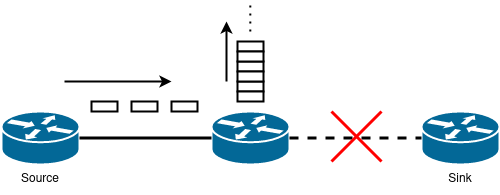
\includegraphics[width=1\linewidth]{storeandforward_down}
  \caption{The link is down so the intermediate router buffers packets instead of dropping them.}
  \label{fig:saf_down}
\end{subfigure}
\begin{subfigure}{.65\textwidth}
  \centering
  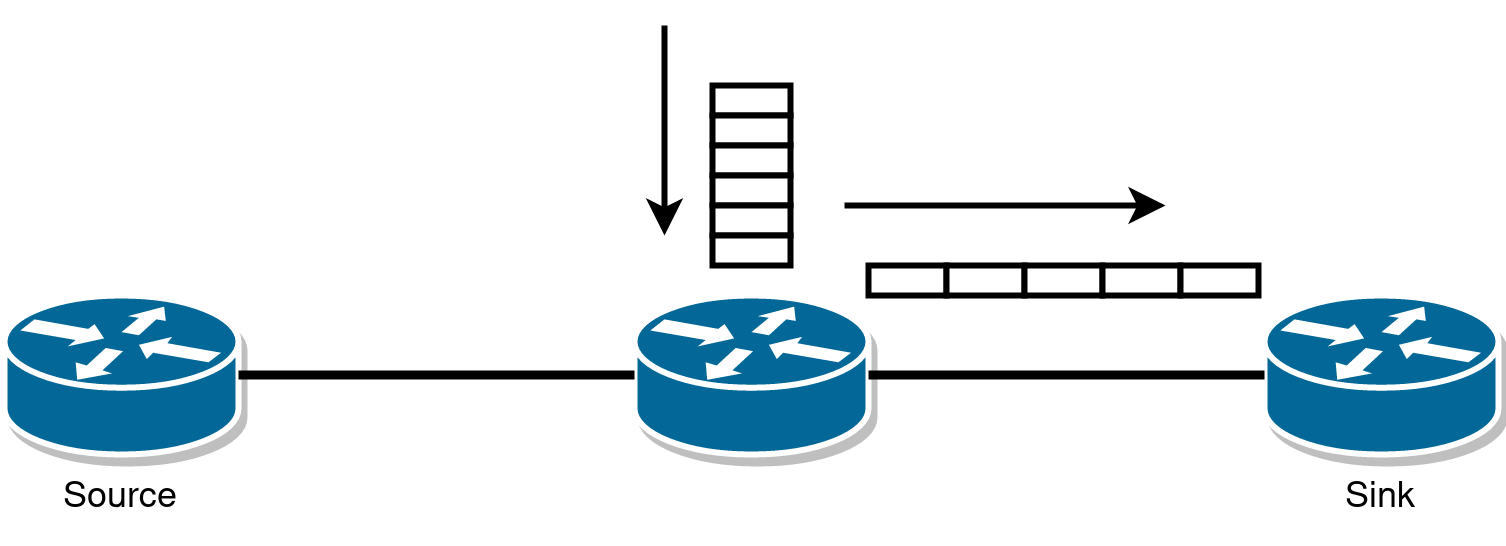
\includegraphics[width=1\linewidth]{storeandforward_up}
  \caption{Once the link comes back up the buffered packets are sent.}
  \label{fig:saf_up}
\end{subfigure}
\caption{Using the store-and-forward technique reduces packet drops, reducing the retransmission load on the source.}
\label{fig:saf}
\end{figure}
\end{minipage}
\end{center}

When we consider multiple link failures occurring along a path at once, the total time where an end-to-end connection exists can drop greatly. When every router along the path has store-and-forward capabilities, our network becomes far more resistant to failures, giving the best possible service to users given the environment.

\begin{center}
\begin{minipage}{0.9\textwidth} \centering
\begin{figure}[H]
\centering
\begin{subfigure}{.45\textwidth}
  \centering
  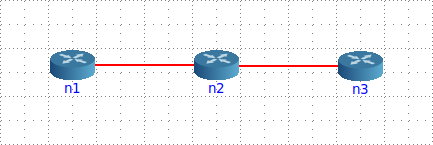
\includegraphics[width=1\linewidth]{pathalogical_topology}
  \label{fig:pathalogical_topology}
\end{subfigure}%
\begin{subfigure}{.55\textwidth}
  \centering
  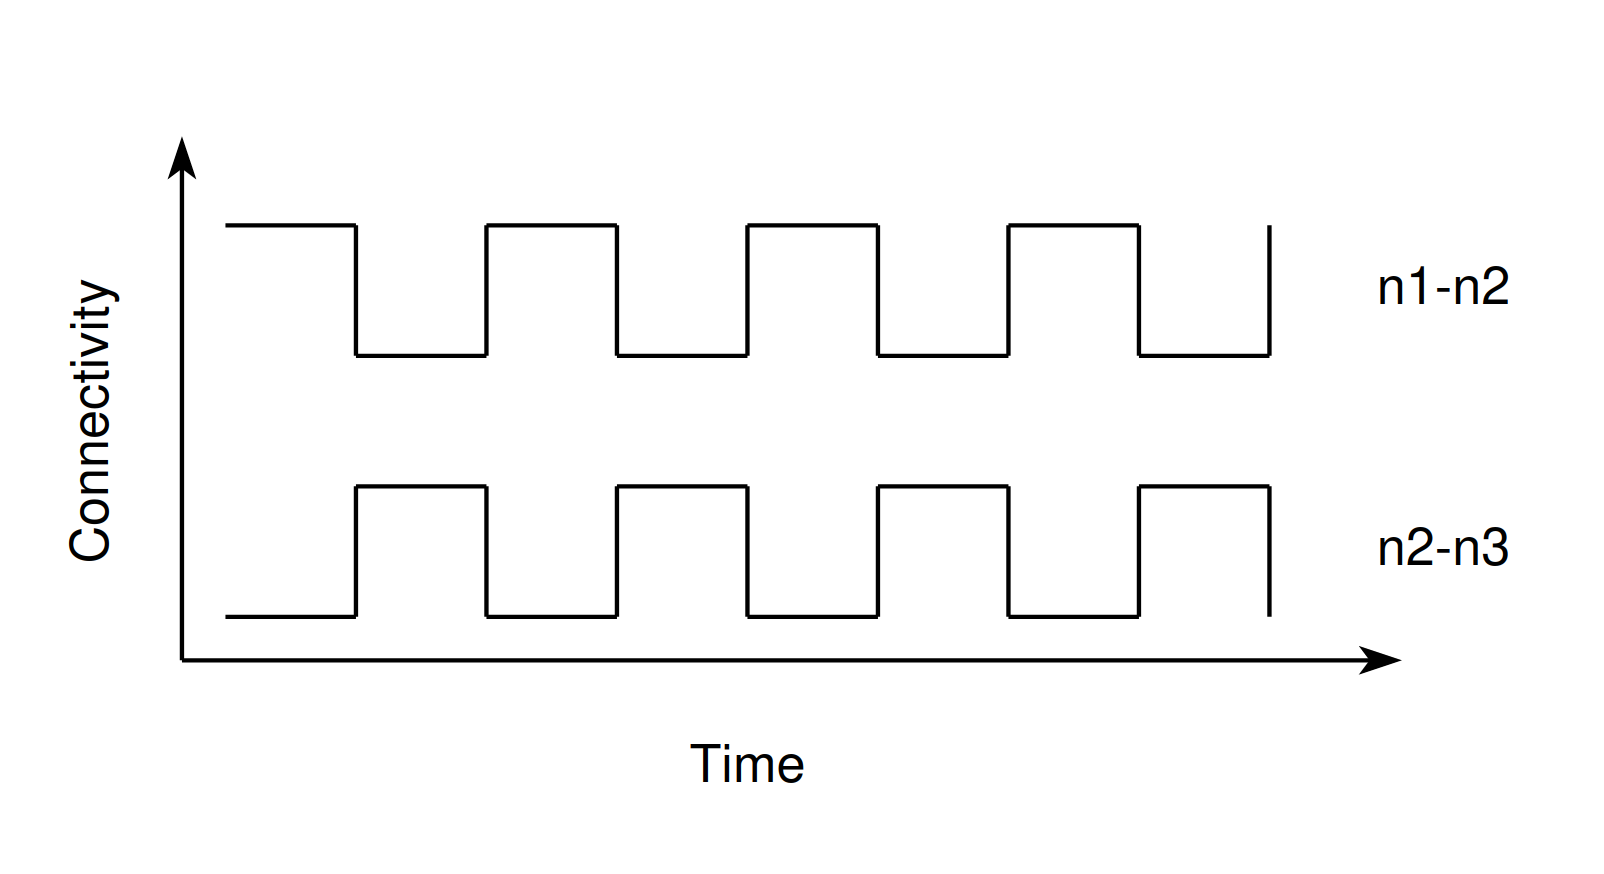
\includegraphics[width=1\linewidth]{pathalogical_graph}
  \label{fig:pathalogical_graph}
\end{subfigure}
\caption{Pathalogical case where a store-and-forward technique allows packets to be delivered despite no end-to-end connection. Traditional techniques will drop all packets.}
\label{fig:pathalogical}
\end{figure}
\end{minipage}
\end{center}

\section{Objectives of the Project}

This project compares the performance of a protocol using traditional link-state routing with a modified version implementing delay-tolerant features. To have control over the behaviour of the protocols both are implemented from scratch in C, with the design based off of the OSPF protocol. The evaluation focuses mainly on the drop rate of packets along with the delay of packet arrivals. We do the evaluation by running the protocols on an industry-grade network emulator that provides a realistic testing environment with full control over the network properties.

\subsection{Results}

DTLSR greatly decreases the drop rate of packets over networks with frequent partitions. Even when a higher-delay backup link exists which LSR can switch onto, our evaluation shows that DTLSR still reduces the packet drop rate by at least half. We also experimentally show cases with multiple link failures where LSR achieves zero packet delivery, but DTLSR delivers more than 70\% of packets.

\section{Related Work}

% JCW cites needed  -- try adding 'survey' to your search terms because those shoudl cover most of the existing work within them.
% jcw: note --- is for em dash, not -
% OTherwsie excellent paragraph explaining why is is related but not usefu.
There has been much research into `mobile ad-hoc networks', where mobile nodes physically move around and have intermittent and unpredictable connectivity with other nodes. This requires a dramatic change in network protocol design, but for our situation it is not necessary. Link failures in a mobile network are usually due to topology changes, but networks in developing regions have largely static topologies with modem or satellite links where link failures, mostly due to congestion or unreliable power, do not imply that the topology has changed. When the failure is resolved the topology will be the same as before, thus we are able to use a well-understood link-state paradigm with comparatively minor modifications, making deployment far easier and minimising wasted resources from unnecessary features.



\chapter{Preparation}

\section{Comparison to Retransmission-based Solutions}
\label{sec:retransmission}

An alternative solution to the problem of delay-tolerance  is for the source to retransmit packets that it believes have been dropped. This may be done in an end-to-end manner via signalling, such as TCPs fast retransmit, or by timeout in the absence of a signal, such as TCP timeout on the absence of receiving an ACK.

For the environment we are concerned with where links go down for extended periods of time, we are naturally only able to consider the second case, where the absence of a signal indicates loss. We could consider the first case if intermediate routers before the failed link were able to signal, but for this we are considering session-level TCP-like protocols that are in common use.

If we set the retransmission timeout to $\alpha$ seconds, and the time the link is down to $\beta$ seconds, then assuming we send the packet as soon as the link goes down and that we have a best-case of zero propagation delay, we retransmit the packet $N$ times (causing a total of $N$ packet drops including the initial transmission), shown in Equation~\ref{eq:retransmission_n}. Once the link comes back up we have an error where we wait for $E$ seconds before transmitting the packet that actually gets through, shown in Equation~\ref{eq:retransmission_e}.

\begin{minipage}{0.35\textwidth}
\begin{equation} \label{eq:retransmission_n}
N = \Big\lceil\frac{\beta}{\alpha}\Big\rceil
\end{equation}
\end{minipage}%
\begin{minipage}{0.65\textwidth}
\begin{equation} \label{eq:retransmission_e}
E = \alpha N - \beta = \alpha \Big\lceil\frac{\beta}{\alpha}\Big\rceil - \beta
\end{equation}
\end{minipage}

The error $E$ is due to the fact that we are not responding to the changing state of the link, but just periodically `polling' until it works. This is a fundamental limitation of using an end-to-end technique to detect an intermediate failure along the path, and is thus one of the reasons we chose to explore the network-layer technique of packet buffering instead. As the router detects the link coming up, it can immediately respond by sending the buffered packets, minimising the time wasted and minimising the end-to-end packet delay.

As well as having a larger delay, we see in the value of $N$ and in the name of the technique itself that the sending source must continually retransmit packets, making poor use of valuable processor time and memory. Packet buffering techniques drastically minimise this, with the source most of the time only having to transmit the packet once even when the link is down.

As shown in the evaluation packet buffering techniques do still have a small number of packet drops and so some end-to-end retransmission is needed, but when the link comes back up we are free to use an explicit signalling technique from the destination endpoint to identify dropped packets, such as TCPs triple-ACKed fast retransmit, minimising the amount of retransmission that the source needs to do.

\section{Common Open Research Emulator (CORE)}

CORE is a network emulator that models nodes as lightweight Unix virtual machines, complete with filesystems and network interfaces. It comes out of the US Naval Research Laboratory and was developed by Boeing Research and Technology. In Figure~\ref{fig:core_topology} we see an example topology in the CORE GUI, and in Listing~\ref{core_filesystem} we see an example of a virtualised file-system of one of the nodes; boot scripts and log files of the \texttt{dtlsr} and \texttt{heartbeat} (\texttt{hbt}) protocols are visible. Nodes communicate via virtualised interfaces, connected by bridges emulating physical links. We see an example of this in Listing~\ref{core_interfaces}.

\begin{center}
\begin{minipage}{0.9\textwidth} \centering
	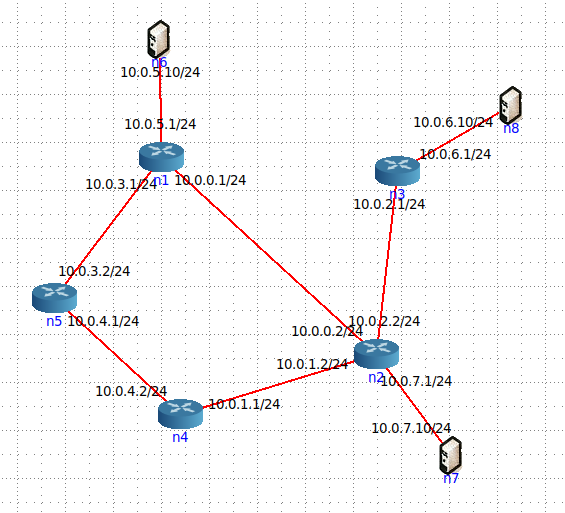
\includegraphics[width=0.65\textwidth]{core_topology}
	\captionof{figure}{Example emulated network in the CORE GUI, showing virtual routers and hosts along with their IP addresses.}
	\label{fig:core_topology}
\end{minipage}
\end{center}

Programs can be written for these nodes and run as Unix processes via a Python API. These processes are then able to send and receive data through the emulated network via standard Unix socket programming. The emulated routers contain default routing protocol implementations, such as OSPFv2 and v3 from the Quagga protocol suite, which can be disabled and replaced by custom implementations. As well as this, standard network testing tools like \texttt{ping} can be run on emulated endpoint hosts, making testing and evaluation of the network simple: in Figure~\ref{fig:core_topology} we could run \texttt{ping 10.0.5.10} from the node \texttt{n7}, sending pings between \texttt{n7} and \texttt{n6}.

Link properties such as delay and loss can be programmatically customised through the Python API. This aids greatly in evaluation, allowing us to simulate network partitions and other network events. In Figure~\ref{fig:core_topology} if we disabled link \texttt{n1-n2} the pings going between \texttt{n7} and \texttt{n6} would have to be rerouted through \texttt{n5} and \texttt{n4}.

An interesting point is that because CORE operates in real-time using the host operating systems clock, the performance of the simulated network is dependent on the performance of the machine it's running on. We therefore take great care to create a reliable and statistically sound testing environment, for example setting processor priority, not running other programs, and taking baseline measurements to compare against. However the clock sharing is also an advantage for evaluation, as when deriving the time between events on different virtual machines we don't need to account for any clock drift; the time difference will be as exact as if they were the same machine. This will make evaluation easier and more accurate, reducing the error.

\begin{minipage}{1\textwidth} \centering
\begin{lstlisting}[label=core_filesystem, frame=tb, caption=Virtualised file-system of the node \texttt{n1}]
ben@ben-laptop:/tmp/pycore.1/n1.conf$ ls -lh
total 40K
-rw-r--r-- 1 root root   98 Apr 16 14:43 defaultroute.sh
-rw-rw-rw- 1 root root    0 Apr 16 14:43 dump_0.pcap
-rw-r--r-- 1 root root  103 Apr 16 14:43 hbtboot.sh
-rw-r--r-- 1 root root    1 Apr 16 14:43 hbt.id
-rw-rw-rw- 1 root root 2.1K Apr 16 14:44 hbt.log
-rw-r--r-- 1 root root  798 Apr 16 14:43 ipforward.sh
-rw-r--r-- 1 root root   91 Apr 16 14:43 dtlsrboot.sh
-rw-r--r-- 1 root root    1 Apr 16 14:43 dtlsr.id
-rw-rw-rw- 1 root root   61 Apr 16 14:43 dtlsr.log
drwxrwxrwx 2 root root 4.0K Apr 16 14:43 var.log
drwxrwxrwx 2 root root 4.0K Apr 16 14:43 var.run
\end{lstlisting}
\end{minipage}

\begin{minipage}{1\textwidth} \centering
\begin{lstlisting}[label=core_interfaces, frame=tb, caption=Virtualised ethernet network interfaces (\texttt{veth}) are connected by bridges.]
ben@ben-laptop:~$ nmcli device status
DEVICE          TYPE      STATE         CONNECTION
b.10.1          bridge    connected     b.10.1
b.11.1          bridge    connected     b.11.1
b.7.1           bridge    connected     b.7.1
b.8.1           bridge    connected     b.8.1
b.9.1           bridge    connected     b.9.1
veth1.0.1       ethernet  unmanaged     --
veth1.1.1       ethernet  unmanaged     --
veth1.2.1       ethernet  unmanaged     --
veth2.0.1       ethernet  unmanaged     --
veth2.1.1       ethernet  unmanaged     --
veth2.2.1       ethernet  unmanaged     --
veth3.0.1       ethernet  unmanaged     --
veth4.0.1       ethernet  unmanaged     --
veth5.0.1       ethernet  unmanaged     --
veth6.0.1       ethernet  unmanaged     --
\end{lstlisting}
\end{minipage}

\section{Software Engineering Tools and Techniques}

\subsection{Requirements Analysis}

The success criteria revolve around creating two routing protocols, and comparing their performance in a number of metrics. In order to meet these criteria, the implementation must include both the tools to run the protocols as well as tools to evaluate it. These can be further split into more specific deliverables,
specified in Table~\ref{table:requirements}.

\begin{table}[H]
\begin{tabularx}{\textwidth}{Xl}
\hline
\textbf{Requirement} & \textbf{Priority} \\
\hline
Implementation of LSR protocol & Fundamental \\
Making delay-tolerant modifications to LSR to produce DTLSR: link metric, packet buffering & Fundamental \\
CORE testing infrastructure: network generation, running commands on virtual nodes, data logging & Fundamental \\
Code for analysing and plotting collected data & Preferable \\
 & \\
\hline
\end{tabularx}
\caption{Project deliverables}
\label{table:requirements}
\end{table}

\subsection{Tools}

\paragraph{Programming Languages:}

I used \textbf{C} because of extensive previous experience in internships and the Part 1B course, and in order to have low-level access to Unix system calls. As well as this industry-grade routing protocols are generally written in C or assembly, and I wanted to emulate this as much as possible. I used \textbf{Python} to interact with the CORE API, for scripting the testing environment used to evaluate and develop the routing protocols. The Python API is the only one provided, thus it was a natural choice. I also used Python extensively to do analyse and plot the collected data.

\paragraph{Libraries:}

I used \textbf{libpcap} and its command-line equivalent \textbf{tcpdump} for buffering received packets and storing them on the router when the outgoing link was down. I used \textbf{tcpreplay} to send the packets buffered by the tools above out onto the outgoing link when it came back up.

\paragraph{Version Control and Backup:}

I used the \textbf{Git} version control tool, with the repository backed up on the \textbf{GitHub} platform. The repository is also backed up on an external hard drive.


\paragraph{Repository Management:}

I used the \textbf{CMake} build system for C, which allows easy inclusion of dependencies such as libpcap and check, and the generation of multiple executables in the same project, even from the same source files. It also provides platform independence. I used the \textbf{Check} unit-testing framework for C.


\paragraph{Other Tools:}

I used \textbf{CORE version 7.5.2} as it provides a reliable network emulation platform for development and evaluation of network protocols. In particular, it allowed me to disable the existing routing protocols and replace them with my own. I used the \textbf{Packet CAPture (.PCAP)} format, a standard file format for packet data, to store the buffered packets on the router until they could be replayed. It was chosen as tcpdump and tcpreplay understand this format natively.


\section{Starting Point}

This project does not build on any other code/project, but only makes use of common tools and libraries such as libpcap, CORE, and matplotlib (for plotting graphs in the dissertation). CORE comes packaged with standard routing protocol implementations of OSPFv2 and v3, however I disable these completely and do not use them as a starting point for my code, neither for inspiration nor code snippets.

\section{Techniques}

Throughout this project an iterative development model was adopted...

\section{Summary}

The concepts and algorithms required for the dissertation were mostly covered in Part IB Computer Networking, but the delay-tolerant protocol modifications were not included in the course and I had no prior experience with them. Previous experience with C came from the Part IB course as well as a summer internship doing embedded development.

\chapter{Implementation}
% JCW : Can we start with something more exciting?  E.g. a brief overview of what you've implemented?
% I think 2 paragraphs explaining what you've implemented would go very well here --- and help the reader navigate this section.

We have implemented two routing protocols, \texttt{LSR} and \texttt{DTLSR}. These are each composed of link-layer systems for detecting link failure and links coming back up, integration of this information into an internal graph representation of the network, and a network-layer mechanism for propagating this information over the entire network.

Also implemented is a way for each router to use this information to generate shortest paths to every other node, aggregating this information to modify the routing table accordingly. Significant effort was put into the delay-tolerant modifications in \texttt{DTLSR}, with a local packet buffering system for link-failure tolerance, and a sophisticated metric for comparing the reliability of links.

\section{Repository Overview}
\begin{minipage}{1\textwidth} \centering
\begin{lstlisting}[label=repository, frame=tb]
dtlsr                        Root
|- configs                   CORE config files
|- include                   Include directory
|  |- algorithm
|  |- network
|  '- process
|- src                       Source directory
|  |- algorithm
|  |- network
|  '- process
|- tests                     Unit tests directory
|  |- algorithm
|  |- network
|  '- process
|- tools                     Custom development tools
'- core-py                   Custom CORE scripts
\end{lstlisting}
\end{minipage}

\begin{itemize}
	\item
	\texttt{algorithm} contains pure algorithms and data structures, for example the graph representation, pathfinding, and heap implementations.

	\item
	\texttt{network} contains functionality for socket manipulation, sending data over the network, and packet listening/replay.
	
	\item
	\texttt{process} contains funtionality for interacting with both CORE and the Unix OS, for example retrieving node information, logging, and manipulating the Unix routing table.
\end{itemize}

The project was implemented almost entirely in C, with CORE-specific scripts in Python. I used the CMake build system and Check unit testing framework.

\section{Link-State Routing Design}

The link-state routing protocol that I implemented is split into two programs, \texttt{heartbeat} and \texttt{lsr}.  Routers run both programs, and hosts run only \texttt{heartbeat}.

% JCW: can we havea  diagram showing the heartbeat and LSR?
% Perhaps with example LSR contents?
\texttt{heartbeat} sends periodic heartbeat messages to all neighbouring nodes, notifying them that the connecting link is still up. The message is received by \texttt{lsr}. Hosts run \texttt{heartbeat} to notify their gateway router of their existence, so that the router can advertise the corresponding route.

\texttt{lsr} implements the bulk of the protocol. It maintains the link-state graph representation of the network, manipulates the node's routing table, and sends link-state announcements (LSAs) to neighbours in response to detected changes in the network. When we say a link is UP or DOWN we mean the router's logical link-state representation of the network, which is a `lagged' view of its real state. The event loop of \texttt{lsr} is shown in Figure~\ref{fig:flowchart_lsr}.

Changes are detected in one of three ways:
\begin{enumerate}
	\item
	A heartbeat message is received from a neighbour with a DOWN link. We set the link to be UP.
	
	\item
	A heartbeat is not received in time from a neighbour with an UP link. We set the link to be DOWN.
	
	\item
	An LSA is received from a neighbour. If they have any information more recent that ours that causes a change to our network representation when merged in, a change is detected.
\end{enumerate}

\begin{center}
\begin{minipage}{0.9\textwidth} \centering
	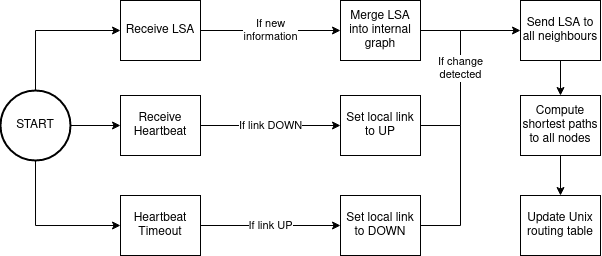
\includegraphics[width=0.9\textwidth]{flowchart_lsr}
	\captionof{figure}{Event loop of \texttt{lsr}, showing responses to different events.}
	\label{fig:flowchart_lsr}
\end{minipage}
\end{center}

Both programs lend themselves to an event-driven design, and so I used file descriptors multiplexed with the \texttt{select} Unix system call to detect and respond to events. The \texttt{select} call blocks the process from running until one of the specified file descriptors is ready to be used, at which point the OS gives the process back control along with information about which file descriptor is ready. Using this we can implement a coarse event system. As examples, receiving socket file descriptors trigger as `ready' when data has arrived and is ready to be read, and timer file descriptors trigger as `ready' when the timer has expired. One can see how these can be composed to create a responsive distributed protocol that uses system resources efficiently, rather than just spinning waiting for something to happen.

Heartbeats and LSAs are received on sockets with distinct ports, allowing them to be differentiated easily by the Unix socket API at the UDP layer. While these are purely link-level communications and as such do not require UDP or even IP information, the socket API is an easy abstraction to use and allows me to reuse code from other parts of the codebase, minimising the possibility of introducing bugs.

A heartbeat message is a UDP packet with only header, no payload. An LSA is a UDP packet whose payload is the sending node's graph representation of the network, simply copied into the payload using \texttt{memcpy}.

We send LSAs to our neighbours whenever we detect a change in the network, propagating link-state information as quickly as possible to minimise convergence time. We also send only when we detect changes with respect to our knowledge of the network so that we don't cause infinite looping of updates.

\subsection{Graph Merging}

On receiving an LSA from a neighbour, we must carefully merge the neighbour's representation of the network into our own, only taking the most recent information. We see in Figure~\ref{fig:lsa} an example of a merge.

\begin{center}
\begin{minipage}{0.9\textwidth} \centering
	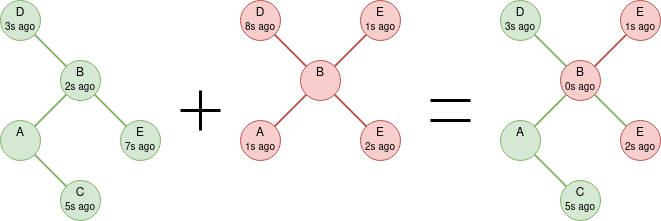
\includegraphics[width=1\textwidth]{lsa}
	\captionof{figure}{Node A receives an LSA from node B, and merges it in to get the most up-to-date view of the network. Blue nodes and links are from A, yellow from B.}
	\label{fig:lsa}
\end{minipage}
\end{center}

To make merging simple we treat every node as independent, in particular having the node's list of neighbours included in the node's data structure rather than having a separate list of links indexed by 2-tuples of node IDs. While this doubles the memory cost of a link as we represent it with two directed edges rather than a single undirected one, it means that merging becomes a simple independent pairwise comparison between nodes of the same ID to pick the one with the most recent timestamp, which has an $O(n)$ time complexity.

When we have successfully merged our neighbour's view of the network into our own, any LSAs that we send will contain this information, thus propagating the global link-state information across the network.

\subsection{Local and Global Link-State}

We have two levels of representation for our network representation: a minimal global representation of the entire network and a detailed representation of the immediate neighbourhood of the local node. We use the detailed local state to derive metrics for the global state graph that we can efficiently share with other routers.

For each node in the global graph, we store for each link information like the source IP, neighbour destination IP, the status of the link, the derived metric associated with the link, and a timestamp specifying how old our knowledge of that link is, for merging purposes.

The local graph consists solely of our node along with more in-depth information about links connecting us to our immediate neighbours. Along with all of the information contained in a global node, we also have for each link a timer for timing out heartbeats and the interface which that link goes out on. We take the locally-derived information and feed it into the global graph, which then gets shared with the rest of the network via LSAs.

The data structures for each are detailed in full in Listing~\ref{node_data_structs}, with a partial example described by Figure~\ref{fig:node_ex} and Listing~\ref{node_ex_listing}. The global graph is an array of \texttt{Node}s, and the local graph is a single instance of \texttt{LocalNode}, representing ourselves.

\begin{center}
\begin{minipage}{0.9\textwidth} \centering
	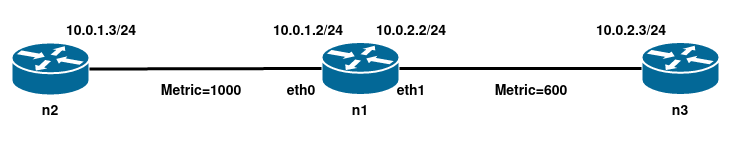
\includegraphics[width=1\textwidth]{node}
	\captionof{figure}{The data structure of node \texttt{n1} is described in Listing~\ref{node_ex_listing}.}
	\label{fig:node_ex}
\end{minipage}
\end{center}

\begin{minipage}{1\textwidth} \centering
\begin{lstlisting}[language=C, label=node_ex_listing, frame=tb, columns=fullflexible, caption=Psuedocode for some fields of \texttt{Node} and \texttt{LocalNode} filled in node \texttt{n1}.]
Node fields:
 neighbour_ids = [2, 3]
 neighbour_ips = [10.0.1.3/24, 10.0.2.3/24]
 source_ips = [10.0.1.2/24, 10.0.2.2/24]
 link_statuses = [UP, UP]
 link_metrics = [1000, 600]

LocalNode fields:
 interfaces = [eth0, eth1]
\end{lstlisting}
\end{minipage}

% BMA -- C is hard to read, maybe some better way to include this?
\begin{minipage}{1\textwidth} \centering
\begin{lstlisting}[language=C, label=node_data_structs, frame=tb, columns=fullflexible, caption=C source code for \texttt{Node} and \texttt{LocalNode} data structures.]
typedef struct node {
  int id;
  enum NodeState state;
  int n_neighbours;
  uint32_t source_ips[MAX_NODE_FAN];
  uint32_t neighbour_ips[MAX_NODE_FAN];
  int neighbour_ids[MAX_NODE_FAN];
  // Link is UP or DOWN
  enum LinkState link_statuses[MAX_NODE_FAN];
  double link_metrics[MAX_NODE_FAN];
  // Node last update time
  unsigned long long timestamp;
} Node;

typedef struct local_node {
  Node node;
  // Heartbeat timer array
  Timer timers[MAX_NODE_FAN];
  // Outgoing interfaces
  char *interfaces[MAX_NODE_FAN];
} LocalNode;
\end{lstlisting}
\end{minipage}

\subsection{Route Generation}

We generate routes from the link-state graph, computing shortest paths from ourself to every other node using Dijkstra's algorithm. From each shortest path we get the next-hop node, which we add to the routing table along with the destination IP subnet so that the router knows where to forward incoming packets. Along with adding new routes we also delete old stale routes, which have either been made obsolete by a new, better route, or do not exist anymore due to failure.

Dijkstra's algorithm computes paths on a weighted graph, allowing us to choose a metric to judge links against each other. Traditional OSPF uses a bandwidth-based metric, but I chose to use the number of hops in the path instead, as delay is more important than throughput in delay-tolerant networks.

With many destinations we have a large number of routing table entries, but we can reduce this by aggregating routes together that share an outgoing interface and IP prefix. As the routing table operates by prefix matching, we only need to insert the shared prefix into the table, reducing the number of entries required greatly.

Manipulation of the Unix routing table is done through \texttt{ioctl}, a system call for interacting with OS devices through a file descriptor interface. We pass a flag corresponding to route addition or deletion, along with a `\texttt{route}' struct containing the route details.

\section{Delay-Tolerant Modifications}

For the delay-tolerant version of the protocol suite, we replace the \texttt{lsr} executable with \texttt{dtlsr}, keeping \texttt{heartbeat} the same. \texttt{dtlsr} uses mostly the same source files as \texttt{lsr}, with the delay-tolerant modifications enabled by \texttt{\#ifdef DTLSR} preprocessor switches, as shown in Listing~\ref{preprocessor_switch}. \texttt{dtlsr} maintains many of the same implementation design decisions as above with a few additions. We see the modified event loop of \texttt{dtlsr} in Figure~\ref{fig:flowchart_dtlsr}.

\begin{center}
\begin{minipage}{0.9\textwidth} \centering
	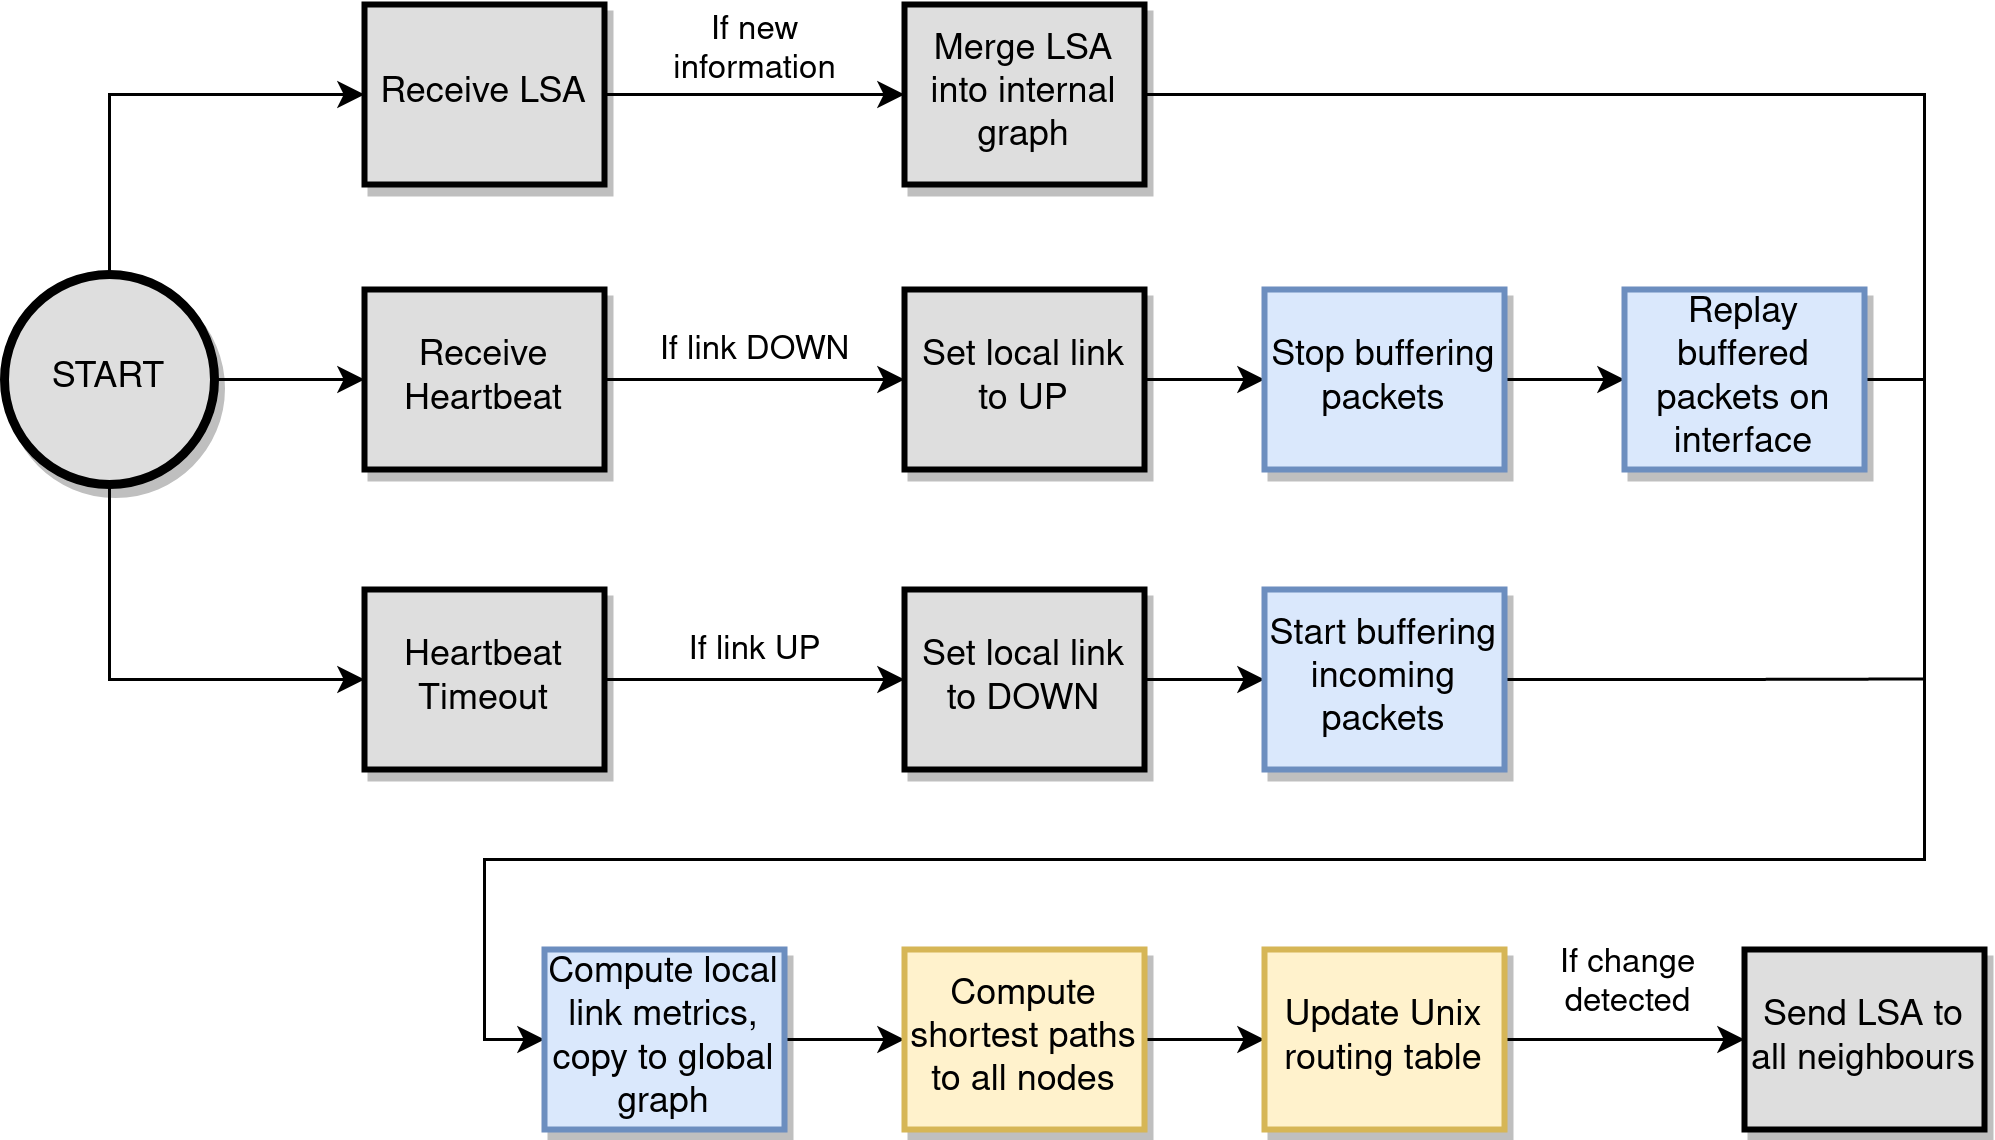
\includegraphics[width=1\textwidth]{flowchart_dtlsr}
	\captionof{figure}{New stages are shown in blue, existing stages that have been modified are shown in yellow.}
	\label{fig:flowchart_dtlsr}
\end{minipage}
\end{center}

\begin{minipage}{1\textwidth} \centering
\begin{lstlisting}[language=C, label=preprocessor_switch, frame=tb, caption=Example of preprocessor switch for DTLSR modifications; the choice of link metric differs in LSR and DTLSR.]
for (int i = 0; i < this->node.n_neighbours; i++) {
#ifdef DTLSR
  // For DTLSR, we use our more complex uptime metric
  this->node.link_metrics[i] =
      ts_compute_metric(&this->ls_time_series[i], now);
#else
  // For LSR, path cost is simply the hop count
  this->node.link_metrics[i] = 1.0;
#endif
}
\end{lstlisting}
\end{minipage}

\subsection{Routing Through Down Links}

In order for other nodes to send us their traffic to go through these down links, we must advertise routes as if the links were up. We take the first step in doing this by modifying the Dijkstra pathfinding algorithm to allow paths to go through DOWN links, which was prevented in the LSR protocol. With all of the paths generated, we proceed in the same way as the LSR protocol, advertising these paths to neighbours via LSAs.

An interesting implementation detail is that we must also add this route to the routers forwarding table. We must do this due to the feedback behaviour of ICMP: if we receive a ping that we must forward on, but are not able to match its destination IP address in our forwarding table, then the kernel will drop the packet and send ICMP `\texttt{Network is unreachable}' response messages back to the sending source. The pings will still be buffered however, and once the link comes back up, they will be sent on to the actual destination which will send back to the source corresponding ping response messages. However the source will not accept these responses as they have already been nullified by the `\texttt{Network is unreachable}' messages, thus making ping unusable for evaluating the network. On the other hand if we add the route to the forwarding table then these erroneous responses will not be generated by the router.

A downside to this is that incoming packets will be sent out of the interface onto the down link, deleting them. As we are buffering these packets as well, when the link comes back up there is a small chance of packet duplication, detailed in Figure~\ref{fig:packet_duplication}, however for testing purposes this is not an issue. To resolve this in a full implementation one would have to modify the behaviour of ICMP in the kernel, as well as potentially other network-layer protocols that have similar behaviour. I wanted to remain in userspace for ease of implementation, so as it has no effect on my evaluation I left it be.

%\begin{center}
%\begin{minipage}{0.9\textwidth} \centering
%	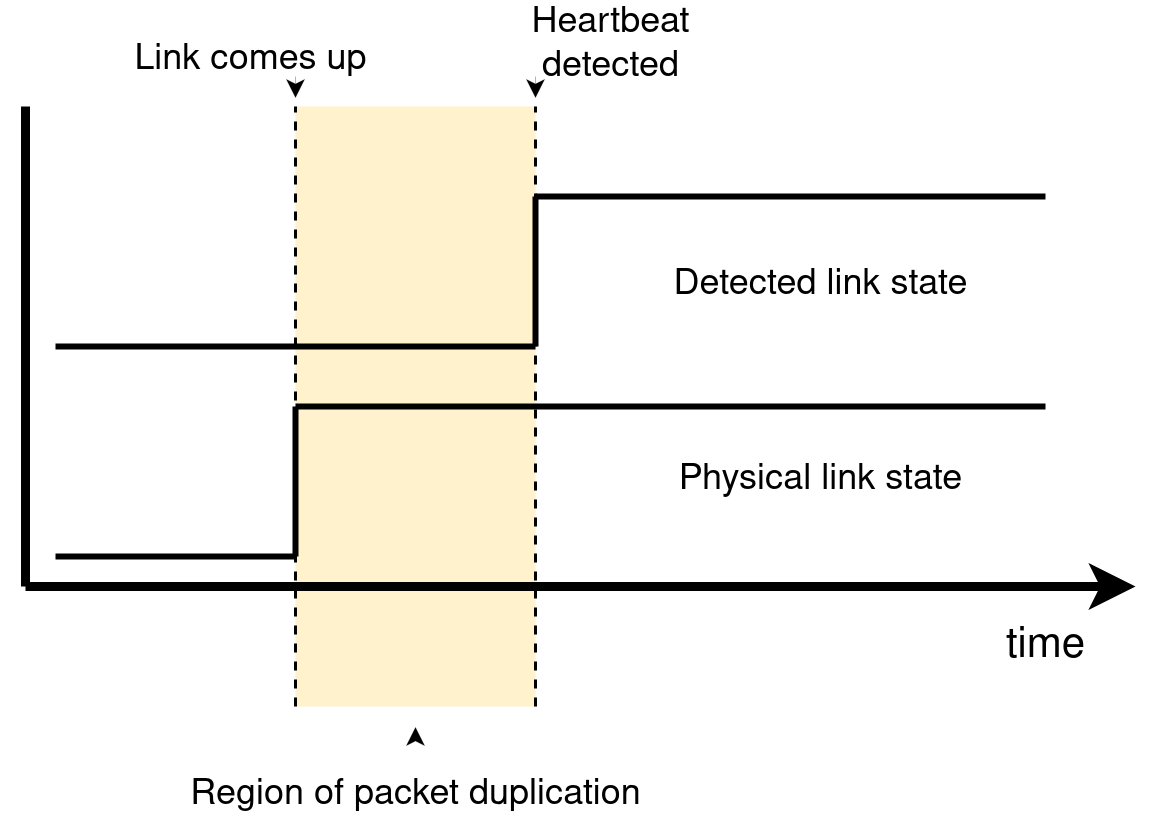
\includegraphics[width=0.8\textwidth]{packet_duplication}
%	\captionof{figure}{Packet duplication is caused by us continuing to buffer packets that are being successfully forwarded on, as we have not yet detected that the link has come up. All packets received in the shown time interval are duplicated.}
%	\label{fig:packet_duplication}
%\end{minipage}
%\end{center}

% JCW: we've switched to we -- that's ok just be consistent
% JCW: careful with this para --- being aware of bugs is good, but no need to advertise yourself as incomplete -- I think this one is good, becaause the bug is interesting --- but I think you should perhaps talk about the benefits of such a fix (e.g. decrease drop rate by X%)
%An interesting edge case is when a link goes down connecting a host with its gateway router. As the host runs \texttt{heartbeat} the router will be aware that the link is down and will buffer any traffic coming in along the advertised route with the host as the destination. However any traffic the host wants to send outwards will not be buffered by itself as it is not running any `delay-tolerant' routing software; the host will have to deal with retransmissions as it will not buffer any data locally.  We could theoretically develop a minimal version of the protocol that runs on hosts and only does buffering to solve this issue.

\subsection{Packet Buffering}

If an outgoing link from a router is down, in our delay-tolerant context the router is responsible for locally buffering incoming traffic that should be going out of the outgoing interface. This is done until either the link comes back up or a better alternative route appears, at which point we send it on.

We use the \texttt{tcpdump} tool for interface listening. When a router knows a connected link is down, it starts listening on all interfaces and dumping received packets to a \texttt{pcap} file, according to a packet filter that only dumps packets going to an IP address that we route to via the down interface, as seen in Figure~\ref{fig:ip_route}. \texttt{tcpdump} is interacted with via the \texttt{libpcap} C library linked in statically with the executable, with the packet filter programmed using the Berkeley Packet Filter (BPF) language. An important optimisation is to place this \texttt{pcap} file on a RAM disk to maximise throughput and minimise latency that can occur when storing files on an SSD or HDD.

\begin{center}
\begin{minipage}{0.9\textwidth} \centering
	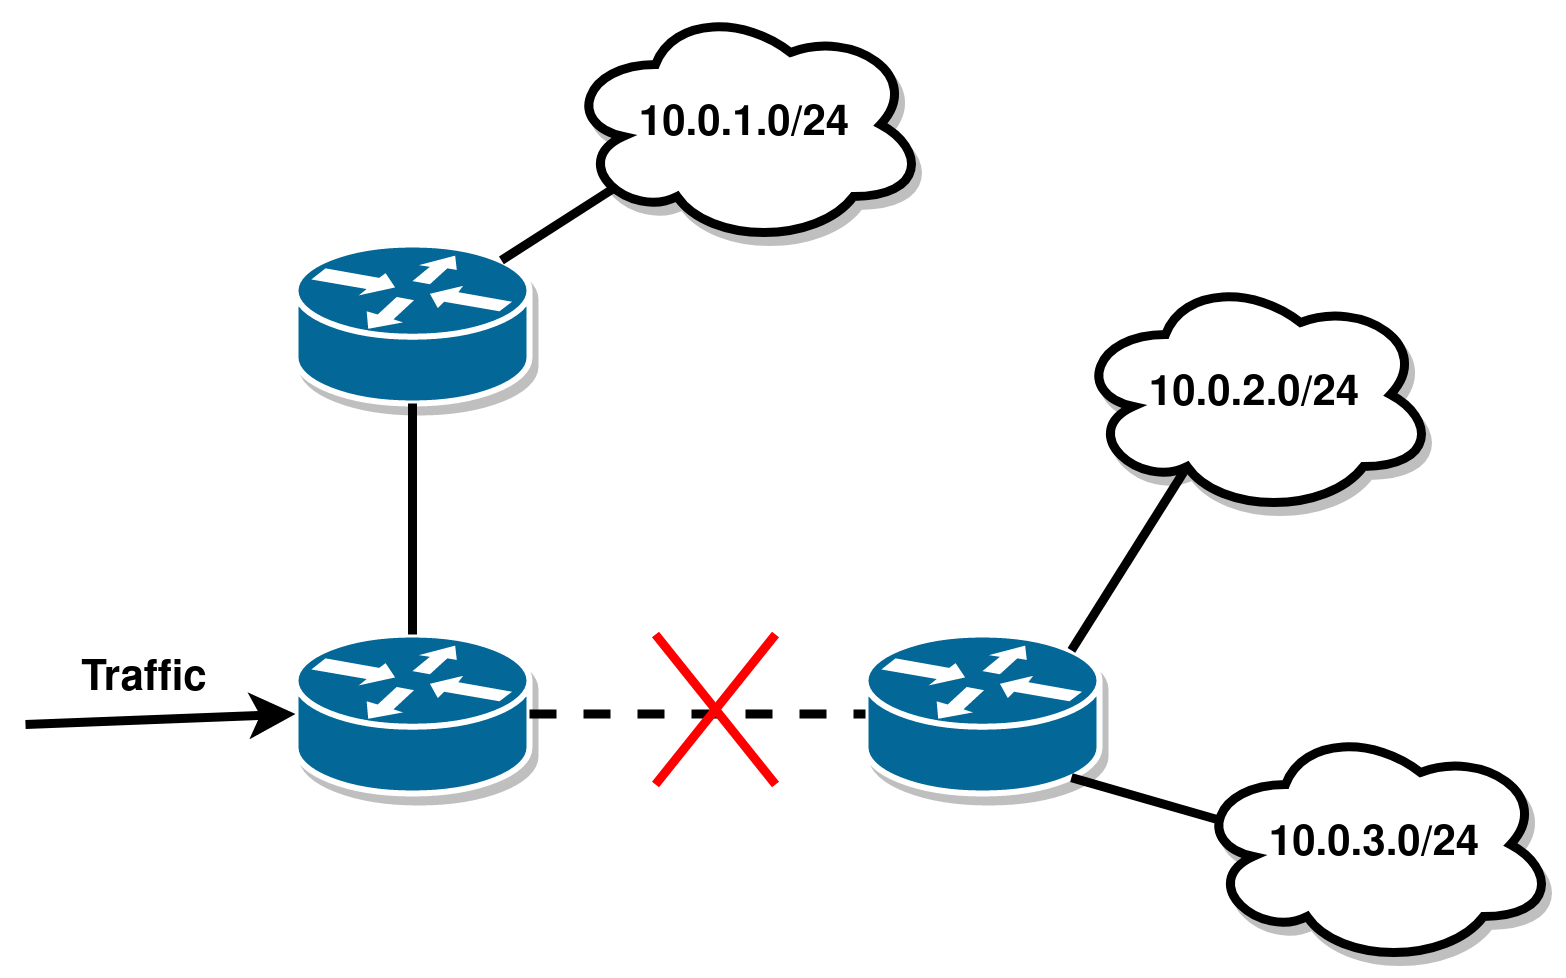
\includegraphics[width=0.6\textwidth]{ip_route}
	\captionof{figure}{The router buffers traffic en-route to the \texttt{10.0.2.0/24} or \texttt{10.0.3.0/24} subnets, as specified by the packet filter. Packets en-route to subnet \texttt{10.0.1.0/24} are forwarded like normal, without buffering.}
	\label{fig:ip_route}
\end{minipage}
\end{center}

When the link comes back up, we stop listening for packets and dumping them to the file, and close the file. From now incoming packets are being sent onto the link correctly so we don't want to duplicate data by buffering then resending it. We make use of a command-line tool, \texttt{tcpreplay}, which allows packets from \texttt{pcap} files to be replayed out of  an interface. We see the command-line call in Listing~\ref{replay_command}. We do this, and then delete the file. Described here is the case of a single failing link, but when multiple links are concurrently failing and coming back up we of course need to be more careful about listening for and replaying only the right data.

\begin{lstlisting}[label=replay_command, caption=\texttt{tcpreplay} command with explanation of arguments, frame=tb]
tcpreplay --topspeed -ieth0 input.pcap

--topspeed - send packets as quickly as possible
-ieth0     - send on interface eth0
input.pcap - .pcap file to read packets from
\end{lstlisting}

% JCW yeah it's a full research project -- a citation would be good ifyou have one.
I chose to use existing tools for packet buffering due to the complexity of this problem, as well as issues with reliability. Even a mature and tested tool like \texttt{tcpdump} still cannot catch all incoming packets at higher speeds; I would have no hope of implementing a suitable alternative in the time I had, and it would likely be a part II project in its own right.

\subsection{Link Metric}

We need some metric to be able to judge the expected delay of a link, in order to compare it to a stable backup link that we can switch onto when appropriate, to minimise the overall delay. This alternative metric is needed only when the link is down, as this is the case when we would want to switch. When the link comes back up we want to send out our buffered packets as quickly as possible, so a metric with some level of hysteresis as we describe below is inappropriate. Through testing it is far more effective to immediately fall back to the standard hop-count metric once the link comes back up.

Assuming that the link will come back up, not switching to the backup link will have no effect on delivery rate as the packets will be buffered, and will reach their destination eventually. However we want to do this in order to reduce the average delay that packets experience, where waiting for the link to come back up will take longer than simply sending via the backup route. We want some level of hysteresis for this so that if failures are historically rare and short-lived, we stick to the primary link.

We use a metric based on the uptime history of the link, computing an integral over the history after exponentially weighting it, as we can see in Figure~\ref{fig:metric}. Integrating over the uptime history tells us how often the link is up, giving us some idea of its reliability over time, and the exponential weighting gives more importance to recent events, making it more responsive. The parameters to the exponential weighting allow us to tune its responsiveness.

Equation~\ref{eq:metric_integral} shows how we compute the integral over one UP period, between times $t_0$ and $t_1$. Our falloff parameter $\alpha$ tunes the metric's responsiveness to changing conditions, increasing it increases the falloff. We compute this integral over each of the UP periods, summing the results together in Equation~\ref{eq:metric_sum}.

\begin{equation} \label{eq:metric_integral}
F(t_0, t_1) = \int_{t_0}^{t_1} f(t)dt = e^{\alpha \cdot t_1} - e^{\alpha \cdot t_0}
\end{equation}

\begin{equation} \label{eq:metric_sum}
F = \sum_{i = 0}^{|\textbf{History}|/2} F(t_{2i}, t_{2i+1})
\end{equation}

The value of $F$ decreases approaching zero as our uptime decreases approaching zero, but we want to inverse this relationship as lower value metrics are chosen with higher preference. As uptime approaches zero, we would like our metric to increase approaching some large value. In the Unix routing table metrics are stored as a 16-bit unsigned value, which has a maximum value of 65,535. We thus want to bound our maximum value below this to prevent integer underflow, which would assign the wrong metric to the route. Our final metric is that shown in Equation~\ref{eq:metric_final}, which has a maximum value of 50,000 when $F$ is 0. Furthermore when the uptime is 100\% the metric takes its minimum value of 1, equal to the hop count of a single UP link that we would use in LSR.

\begin{equation} \label{eq:metric_final}
\textit{metric} = \Big\lfloor\frac{1}{F+0.00002}\Big\rfloor
\end{equation}

\begin{center}
\begin{minipage}{0.9\textwidth} \centering
	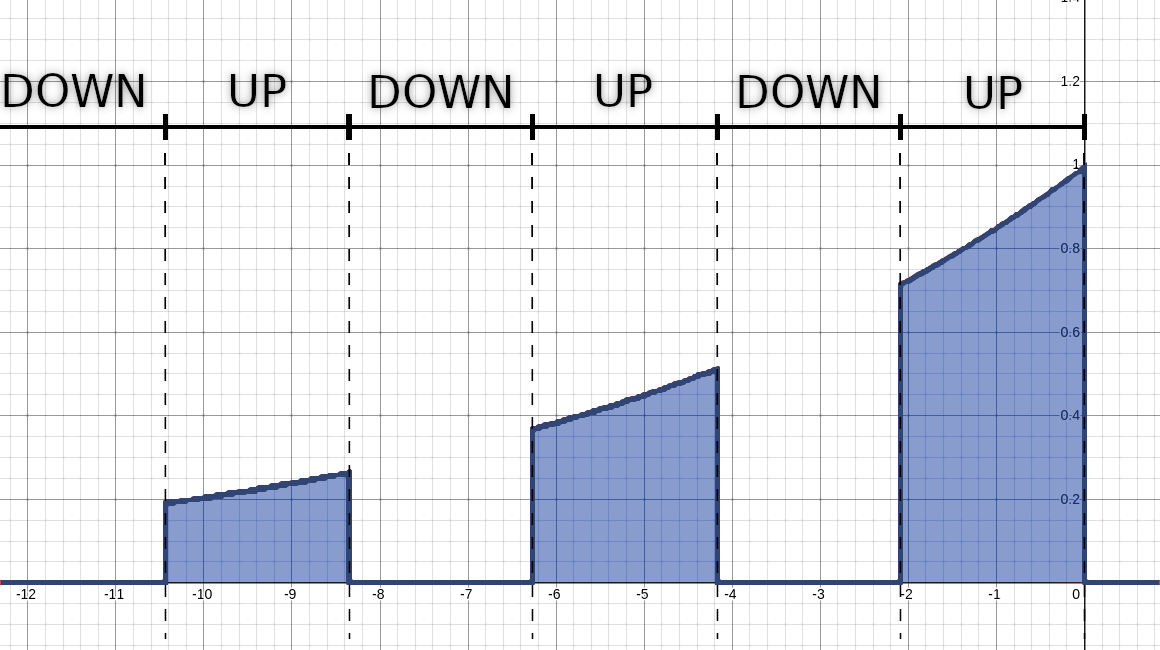
\includegraphics[width=0.9\textwidth]{metric}
	\captionof{figure}{Computing an exponentially weighted integral over the uptime history of the link to give us $F$.}
	\label{fig:metric}
\end{minipage}
\end{center}

We store the uptime history as a circular array of Unix timestamps, each representing the time of an UP or DOWN event. As we know the current state of the link, we can work our way backwards through the array to compute which type of event any given timestamp represents, rather than explicitly storing it. Once the array fills up we start overwriting old events to save memory, however discarding these values has negligible effect on the metric due to the exponential weighting.

The timestamps signify the times of events, but we calculate the metric with respect to our current time. If the last event was a DOWN event, we can imagine the function plot in Figure~\ref{fig:metric} sliding left, changing the value of the metric over time due to the exponential weighting. Because of this changing metric we must periodically update the routing table, as there may be alternative routes with a lower path cost due to the metric increasing.

\section{Implementation Practicalities}

Some parts of the implementation were hard-coded or have inefficient solutions to aid in creating a functional piece of software that could be evaluated more quickly. These are sections that have no impact on the evaluation of the protocol as a solution to the routing problem, or are even completely unrelated to routing in general.

As an example I ran into the issue of `neighbour discovery', where nodes generally use the link-level ARP protocol to discover the existence of neighbouring nodes on their interfaces. The ARP table in CORE proved unreliable, and as this is a link-layer problem unrelated to routing I simply hardcoded all immediate neighbours in configuration files. Implementing actual neighbour discovery would provide no practical benefits to the evaluation, and could even negatively impact it if my implementation was unreliable or had varying performance.

An example of hardcoding is that the memory representation of the link-state graph is statically allocated, i.e. the maximum number of nodes in the network is specified as a compile-time constant. The advantage of this is that it makes indexing and bounds checking very easy and computationally efficient, however we have the twin disadvantages of wasting memory if we are below the maximum number of nodes, and much worse, crashing if the number of nodes increases beyond the maximum. However for the evaluation this is not an issue, as I know beforehand the size and topology of all networks being tested, and can adapt the compile-time maximum as needed. If used in a real, dynamic network, the memory representation would have to be changed to allow dynamic sizing.

While CORE supports IPv6 addressing, I restricted myself to only supporting IPv4 to reduce the unnecessary complexity of supporting another addressing scheme that would have no impact on the performance of the routing protocol, and thus not help my evaluation at all.


\chapter{Evaluation}

The evaluation is done using the CORE emulator. We define a network topology of hosts and routers, with the routers running either the LSR or DTLSR routing protocol, in order to compare the performance of both for a variety of metrics on a variety of different topologies.
% JCW: Add a sentence about why these are the right metrics to measure

We first determine the convergence behaviour of the protocols, to provide a baseline of the testing environment. This is done with LSR, but as DTLSR's system for this is identical the results are valid for both. Convergence time is important for a discussion of delay, as included in the delay is the time taken for routers to respond to changes of the network state; minimising the convergence time should aid us in minimising overall packet delay.

We then do a full comparison of the delay of packet arrivals in LSR and DTLSR in a number of topologies, importantly providing the overall packet loss percentage as well. Packet loss has a critical influence on delay, as the time taken to detect a loss and retransmit can be many orders of magnitude above the time to propagate a packet through the network, drastically increasing the mean delay. We must also consider that information may be spread across multiple packets, meaning that individual packet losses can prevent us from using already received data that depends on it, causing a bottleneck. Thus minimising packet drop rate is critically important.

\section{Convergence}
% JCW: this needs way more subsections --- in general, if you are doing more than 2 paras/subsection, you should think about more subsections --- they just help guide the reader

The convergence time of the link-state protocol, is the time between the state of the graph updating (e.g. a link going down), and that change being detected and incorporated into the routing table of a particular node in the network. As changes are propagated from node-to-node, we expect that convergence time increases as we look at nodes further from the changing link. We will distinguish the convergence time in response to links going down, and links coming back up, as these are detected in different ways. 

Our testing topology is a long chain of routers, shown in Figure~\ref{fig:conv_topology}, with the flapping link at one end and the update messages being propagated down the chain. This gives us a way to detect how long it takes a node to detect the change for each number of router `hops'.

\begin{minipage}{1\textwidth} \centering
	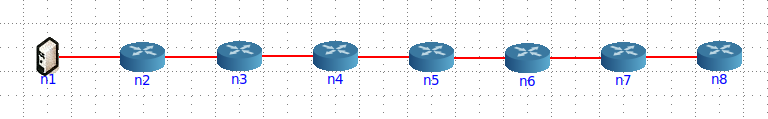
\includegraphics[width=0.7\textwidth]{conv_topology}
	\captionof{figure}{`Convergence' network topology. We flap link \texttt{n1-n2} on the far left.}
	\label{fig:conv_topology}
\end{minipage}

We flap the link using the Python scripting API that CORE provides, waiting 4 seconds between each state change - long enough that we guarantee that all nodes have fully converged before we modify the state again. We log the time when this occurs.

We monitor each node's routing table using the \texttt{route} Unix utility, the output of which is shown in Listing~\ref{route_command}, with a simple Python script that logs the time when we detect that the route corresponding to node \texttt{n1} has either appeared or disappeared from the table, respective to the link being up or down. We can then analyse the data to determine the time between the link changing state, and each node detecting this change and modifying its routing table accordingly.

\begin{lstlisting}[label=route_command, caption=Example routing table of virtualised node, frame=tb]
ben@ben-laptop:~/dtlsr/tools$ python3 vcmd.py n1 route -n
Kernel IP routing table
Destination Gateway  Genmask       Flags Metric Ref Use Iface
0.0.0.0     10.0.1.1 0.0.0.0       UG    0      0     0 eth0
10.0.1.0    10.0.1.2 255.255.255.0 UG    1      0     0 eth0
10.0.1.0    0.0.0.0  255.255.255.0 U     0      0     0 eth0
10.0.2.0    10.0.2.3 255.255.255.0 UG    1      0     0 eth1
10.0.2.0    0.0.0.0  255.255.255.0 U     0      0     0 eth1
10.0.3.0    10.0.3.5 255.255.255.0 UG    1      0     0 eth2
10.0.3.0    0.0.0.0  255.255.255.0 U     0      0     0 eth2
\end{lstlisting}

We do convergence testing with link delays of \SI{1}{\ms} and \SI{100}{\ms}. A link delay of \SI{100}{\ms} is large enough to verify that the convergence time depends on the hop count, from the propagation time, while a delay of \SI{1}{\ms} is what we use for the rest of the evaluation, so it is useful to include as a baseline.  Heartbeats are sent every \SI{200}{\ms}, and the heartbeat timeout is set to \SI{900}{\ms}.

\begin{figure}
\centering
\begin{subfigure}{.5\textwidth}
  \centering
  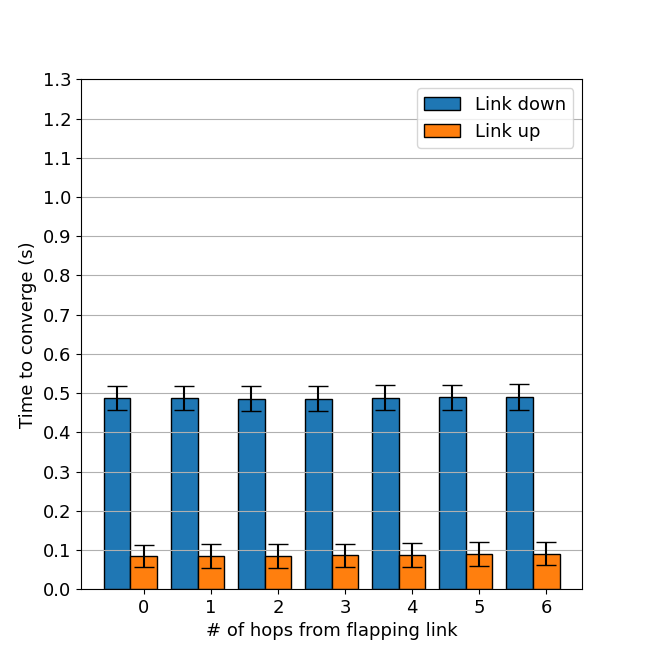
\includegraphics[width=1\linewidth]{conv_1ms}
  \caption{Link delay of \SI{1}{\ms}}
  \label{fig:conv_1ms}
\end{subfigure}%
\begin{subfigure}{.5\textwidth}
  \centering
  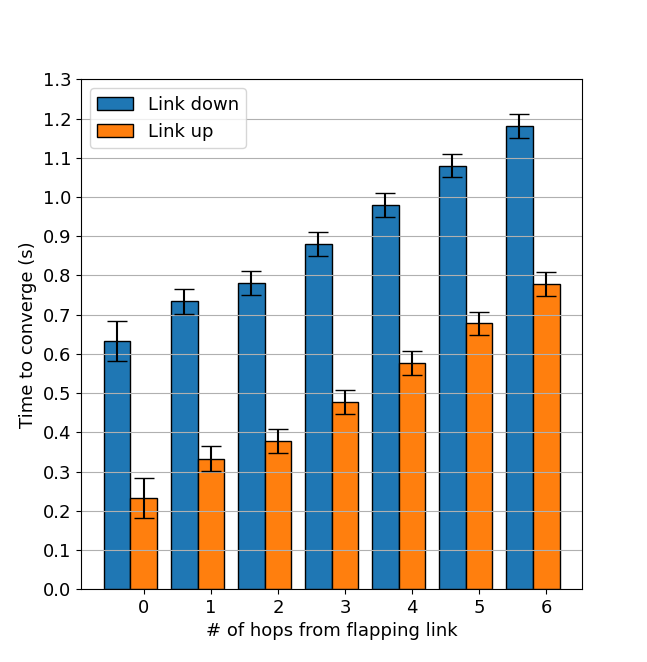
\includegraphics[width=1\linewidth]{conv_100ms}
  \caption{Link delay of \SI{100}{\ms}}
  \label{fig:conv_100ms}
\end{subfigure}
\caption{Protocol convergence times, for both the link going down, and the link coming back up. Error bars are the standard deviation.}
\label{fig:conv}
\end{figure}

\subsection{Results}

In the graphs in Figure~\ref{fig:conv} we see the time between the event occurring and it being detected by the router, depending on the number of hops from the event. We consider the zero-hop node to be that directly attached to the flapping link. In both Figure~\ref{fig:conv_1ms} and \ref{fig:conv_100ms} we see a marked difference between the detection time of the UP and DOWN events, where detection of the link coming up happens much faster than detecting it has failed. This is due to the way these are detected at a link-level, with the former being actively detected by a heartbeat and the latter being passively detected by a timeout. It is then clear that these rely heavily on the particular constants chosen for the heartbeat sending period and the amount of time required for a timeout.

Hop counts of 1 and above rely on the network-layer section of the protocol, with link-state information being sent from node to node. As LSAs are propagated as soon as they are received, we are bounded mainly by the link delay, which we can see in the difference between the higher hop counts of~\ref{fig:conv_1ms} and~\ref{fig:conv_100ms}. In~\ref{fig:conv_1ms} the delay is so small as for each subsequent hop to be almost indistinguishable from the last, but in~\ref{fig:conv_100ms} we see the delay increasing the convergence time for each hop cumulatively, for both UP and DOWN events.

It is interesting to note that subsequent hops depend on the cumulative time added by all previous hops, due to propagation. As the difference between up and down remains close-to constant after the zero-hop node, we can conclude that the network-layer behaviour is the same for up and down, explained by them both depending on the same LSA propagation system.


\section{Delay}

The main body of the evaluation is comparing the distribution of round-trip packet delays for LSR and DTLSR in a number of different network environments, varying topology and failure mode. This demonstrates the different properties of the routing algorithms, showing advantages and disadvantages of both.

We want to evaluate with UDP to minimise any interference that the transport layer may have on testing. We approximate UDP with the Unix \texttt{ping} utility, which despite using ICMP emulates the behaviour of UDP well at higher throughputs, similarly having no flow and congestion control mechanisms. We take the `delay' of a packet as being the round-trip time as computed by \texttt{ping}.

%\begin{lstlisting}[label=route_command, caption=Command-line call used to test delay, frame=tb]
%ping 10.0.x.x -i0.1 -D
%\end{lstlisting}

% JCW: refer to figure in the first sentence of this paragraph
We plot the distribution of delays as a logarithmic CDF plot with the y-axis signifying the proportion of packets, for example shown in Figure~\ref{fig:partition}. When the line goes off the edge of the graph on the right without reaching 1.0 on the y-axis, it shows that the remaining proportion of packets was dropped. I don't include retransmissions as this is a transport-layer responsibility.

Unless specified otherwise, all links have a delay of \SI{1}{\ms}.

% JCW: even this could do with something to break up the length -- see the \paragraph{ } tags maybe?
\subsection{Partial Partition Topology}

Firstly we have a topology with a single central connecting link, \texttt{n1-n2}, that we periodically alternate being up or down; we say that the link is `\textbf{flapping}'. Of note in this topology is that when the link is down it creates a network partition between node subsets \texttt{(n1,n3,n5)} and \texttt{(n2,n4,n6)}.

\begin{minipage}{1\textwidth} \centering
	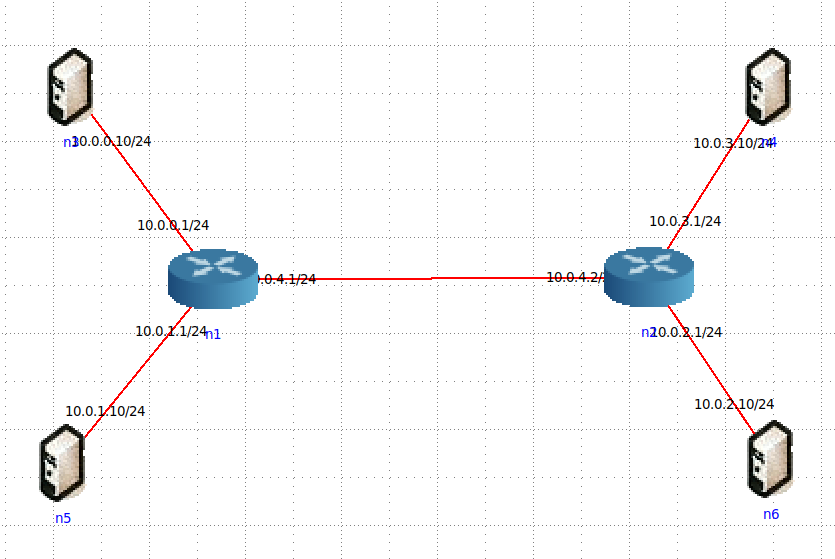
\includegraphics[width=0.5\textwidth]{delay_partition_topology}
	\captionof{figure}{`Partition' network topology.}
	\label{fig:partition_topology}
\end{minipage}

\begin{figure}
\centering
\begin{subfigure}{.8\textwidth}
  \centering
  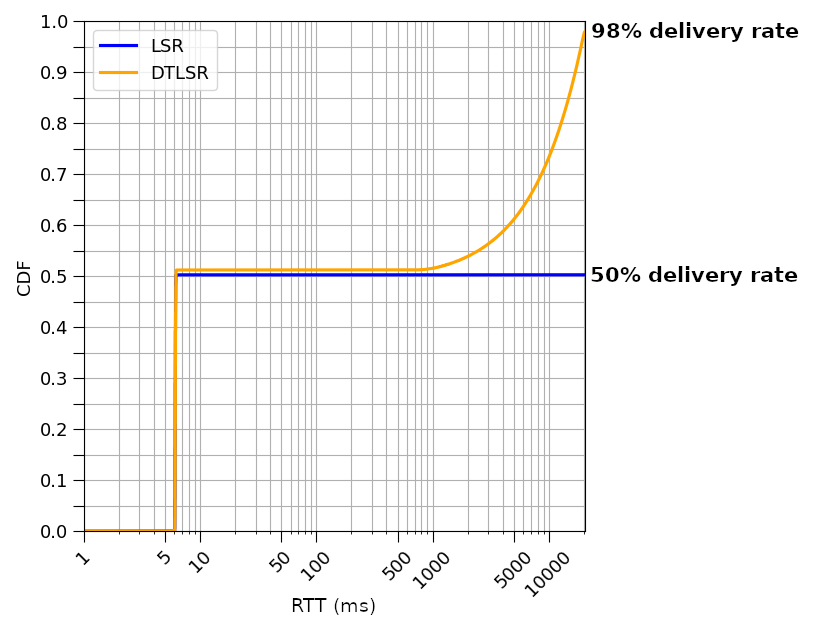
\includegraphics[width=1\linewidth]{delay_partition_flap20}
  \caption{Flapping with period $T=\SI{40}{\s}$ (\SI{20}{\s} up, \SI{20}{\s} down).}
  \label{fig:partition_20}
\end{subfigure}

\begin{subfigure}{.8\textwidth}
  \centering
  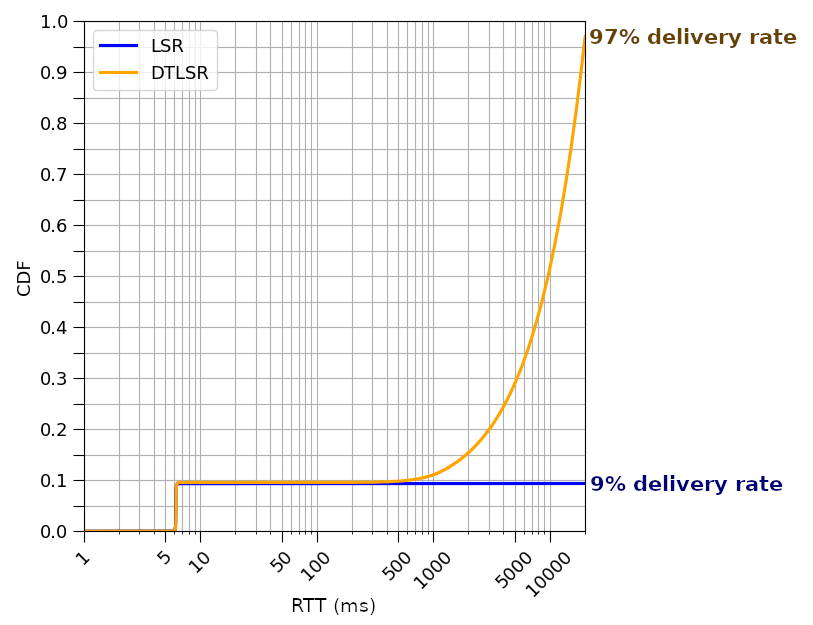
\includegraphics[width=1\linewidth]{delay_partition_flap2_20}
  \caption{Flapping with period $T=\SI{22}{\s}$ (\SI{2}{\s} up, \SI{20}{\s} down).}
  \label{fig:partition_2_20}
\end{subfigure}

\caption{Cumulative distributions of end-to-end delay between \texttt{n5} and \texttt{n6} under different routing algorithms, while flapping link \texttt{n1-n2}.}
\label{fig:partition}
\end{figure}

The results are shown in Figure~\ref{fig:partition}. We see in both cases that LSR successfully delivers a proportion of packets approximately the same as that of the uptime proportion of the link, in Figure~\ref{fig:partition_20} it is up half of the time so we get 50\% delivery, and in Figure~\ref{fig:partition_2_20} it is up one tenth of the time so we get a 9\% delivery rate. We can attribute the 1\% discrepancy to packet drops that will be explained below. DTLSR achieves a drastically higher delivery ratio in both cases due to packets being buffered at the router before the failure, then forwarded on when it comes back up.

In both plots the packets can be split into two groups. For the first group both LSR and DTLSR have a constant delay of \SI{6}{\ms}. For LSR the second group of packets are dropped, whereas for DTLSR their delay increases linearly (showing as an exponential curve in the $\log x$-$y$ graph). The first group is due to the link being up the described proportion of the time of the time, so all packets sent in this period take approximately the same time to arrive, taking a round-trip journey over three links (\texttt{n5-n1-n2-n6}) each of \SI{1}{\ms} delay. The second group is a little more subtle, and is due to the packet buffering and replaying behaviour. \texttt{ping} sends packets at a constant interval but the buffered packets are replayed all at once when the link comes back up, thus the earlier that a ping is sent in the link-down period, the greater time delay there will be between the client sending the packet and receiving a reply.

This variability in delay can be undesirable, but it is not something that can be fixed as partitioning is a fundamental property of the network that we can't work around. Even a perfect retransmission protocol would run into the same variability issue, retransmitting all of the dropped packets as soon as the link came back up. Users of the network should take this into account with the applications that they decide to run on it, and ensure that there are not strict low-latency requirements with applications like video conferencing or real-time games.

\begin{figure}
  \centering
  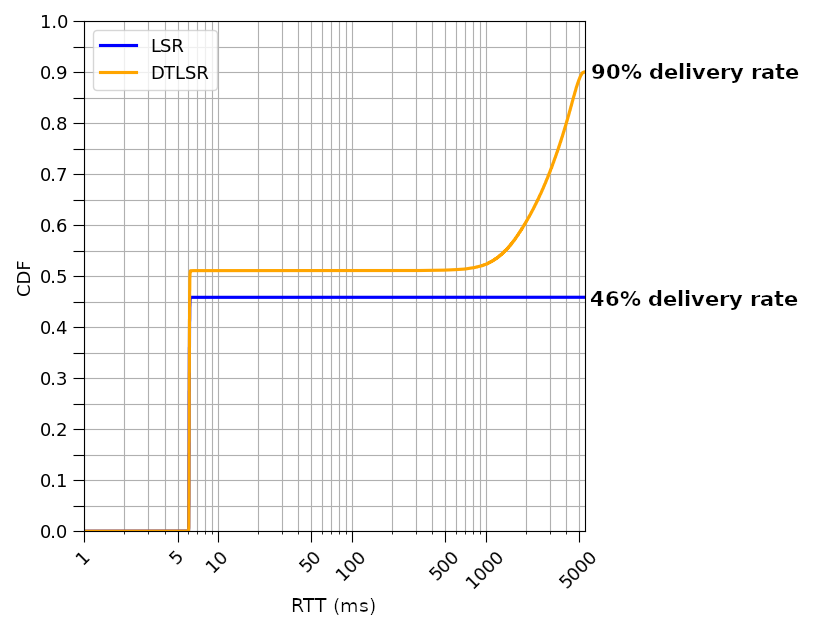
\includegraphics[width=0.8\linewidth]{delay_partition_flap5}
  \caption{Flapping with period $T=\SI{10}{\s}$ (\SI{5}{\s} up, \SI{5}{\s} down).}
  \label{fig:partition_5}
\end{figure}

Comparing Figures~\ref{fig:partition_5} and \ref{fig:partition_20}, we see that increasing the flapping frequency creates a higher drop rate overall for both protocols, which can be explained by considering that when a link goes down it takes time for the router to detect this change, in which time any incoming packets are sent out of the interface and are summarily deleted. It is only once the state change is detected that we change our routing tables or start buffering packets, for LSR and DTLSR respectively. The higher the flapping frequency, the higher proportion of time we spend in these `boundary' periods, and thus the more packets we drop for both LSR and DTLSR.

% good --- this should be in a more prominent location --- I would start with this at the begininf of the section ---e.g. toplogy descriptionn, motivation, results, exlanation of features?
This network topology is consistent with those seen in remote regions even in developed countries, where there is a single main link being relied on. If that link becomes unreliable, then we have shown that using a delay-tolerant routing protocol greatly increases the proportion of packets delivered. One could imagine a situation where the link is only up for a small proportion of the total time, instead of half-and-half, in which case DTLSR would show an even greater advantage over LSR.


\subsection{Full Partition Topology}

Our second topology shown in Figure~\ref{fig:full_partition_topology} is similar to the above `partition' topology, but instead partitions the network with two links in sequence that have anti-correlated failures as shown in Figure~\ref{fig:full_partition_graph} --- when one is up, the other is down. Thus there is never any end-to-end connection and the network is technically always partitioned, but using the `store-and-forward' mechanism some packet delivery can be achieved. This is not as ridiculous a case as it may seem. If a region has unreliable or limited power, there may only be sufficient power to turn on a subset of the routers at a time, likely in an unpredictable pattern.

\begin{figure}[H]
\centering
\begin{subfigure}{.5\textwidth}
  \centering
  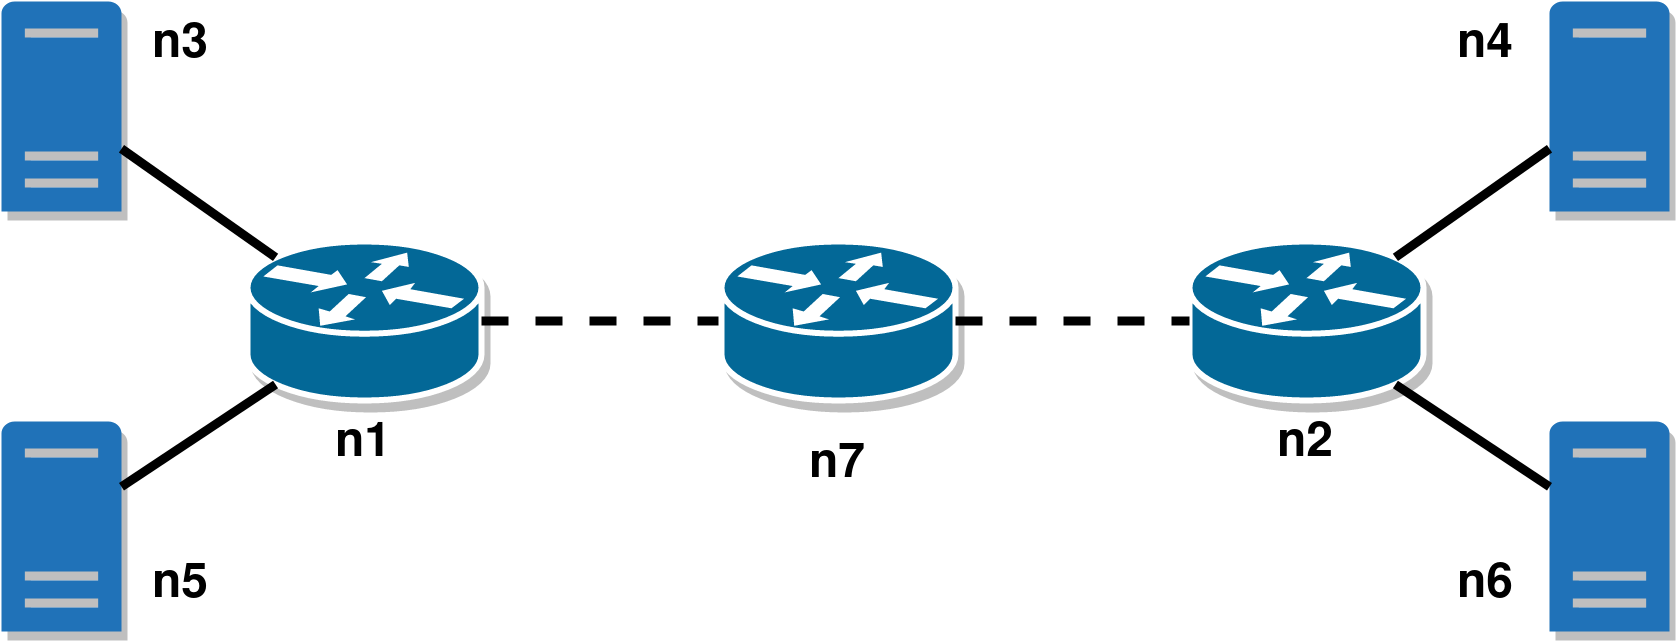
\includegraphics[width=1\linewidth]{delay_full_partition_topology}
  \caption{}
  \label{fig:full_partition_topology}
\end{subfigure}%
\begin{subfigure}{.5\textwidth}
  \centering
  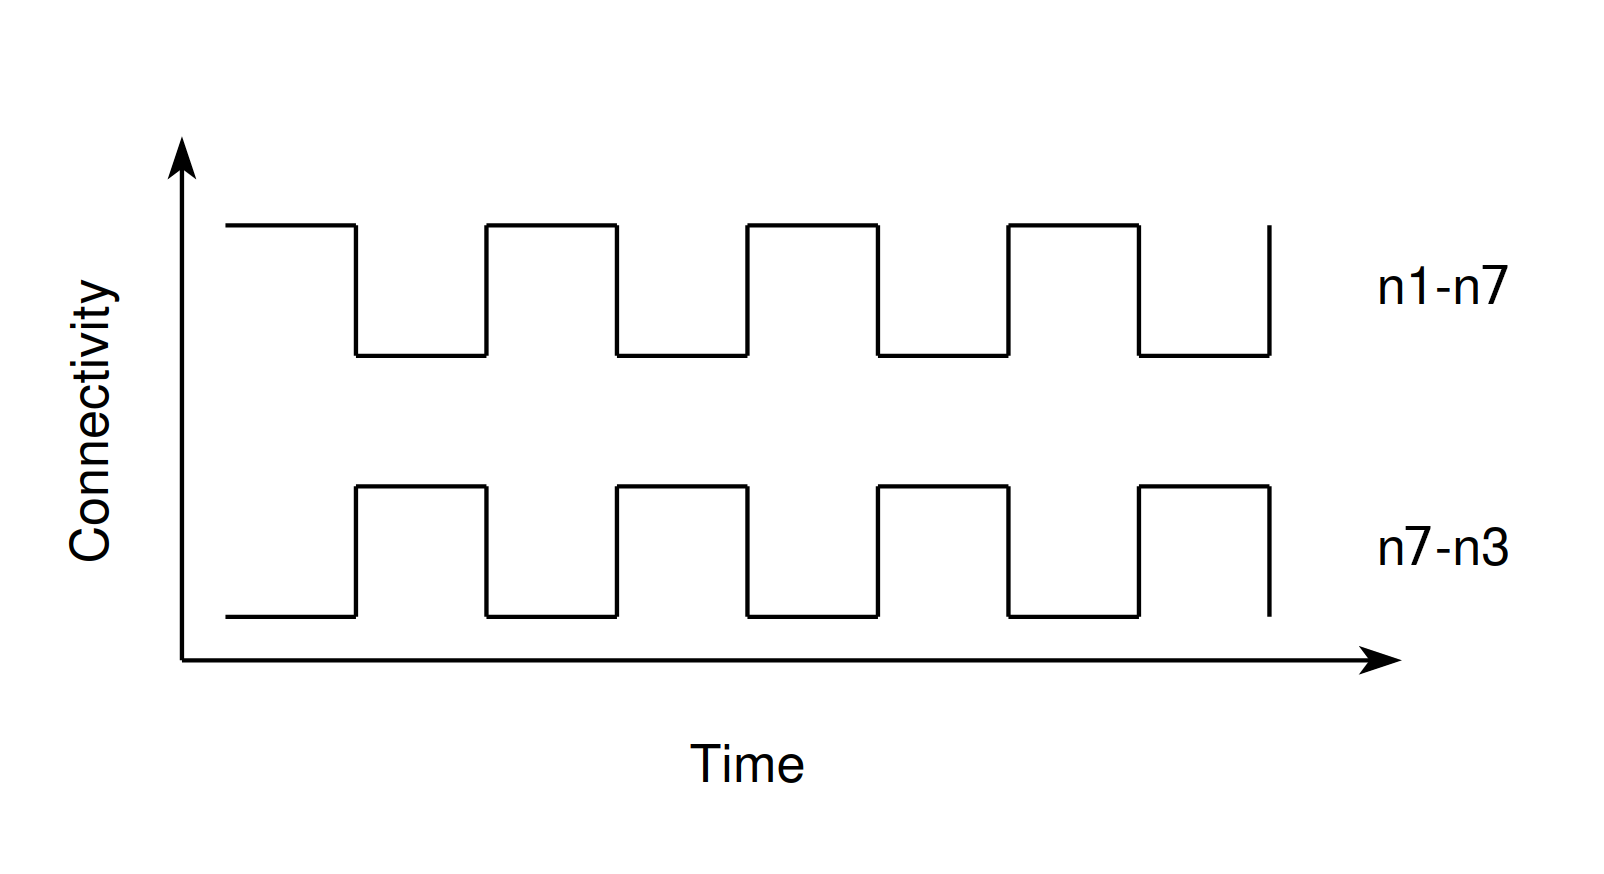
\includegraphics[width=1\linewidth]{delay_full_partition_graph}
  \caption{}
  \label{fig:full_partition_graph}
\end{subfigure}
\caption{`Full partition' network topology with anti-correlated link failures.}
\label{fig:full_partition}
\end{figure}

\begin{figure}[H]
\centering
\begin{subfigure}{.8\textwidth}
  \centering
  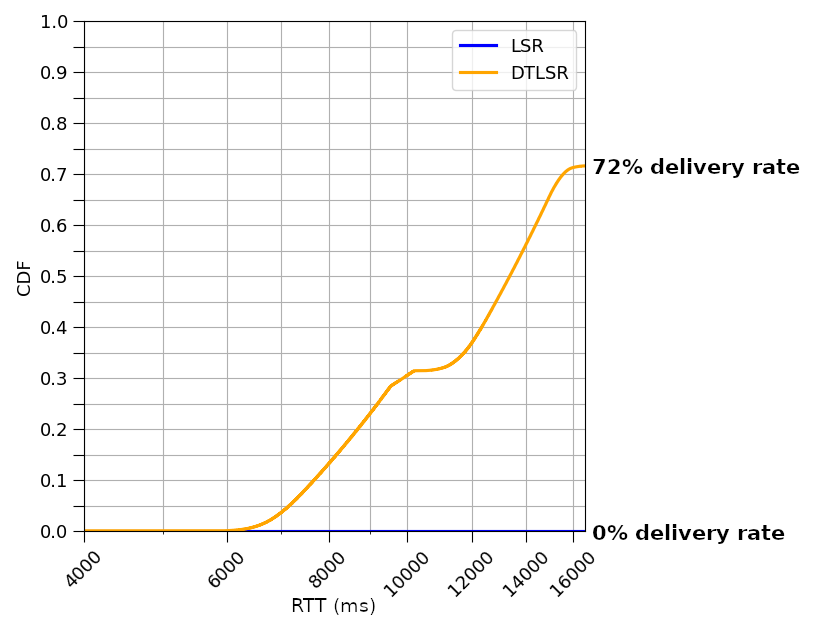
\includegraphics[width=1\linewidth]{delay_full_partition_flap5}
  \caption{Flapping with period $T=\SI{10}{\s}$ (\SI{5}{\s} up, \SI{5}{\s} down).}
  \label{fig:full_partition_flap5}
\end{subfigure}

\begin{subfigure}{.8\textwidth}
  \centering
  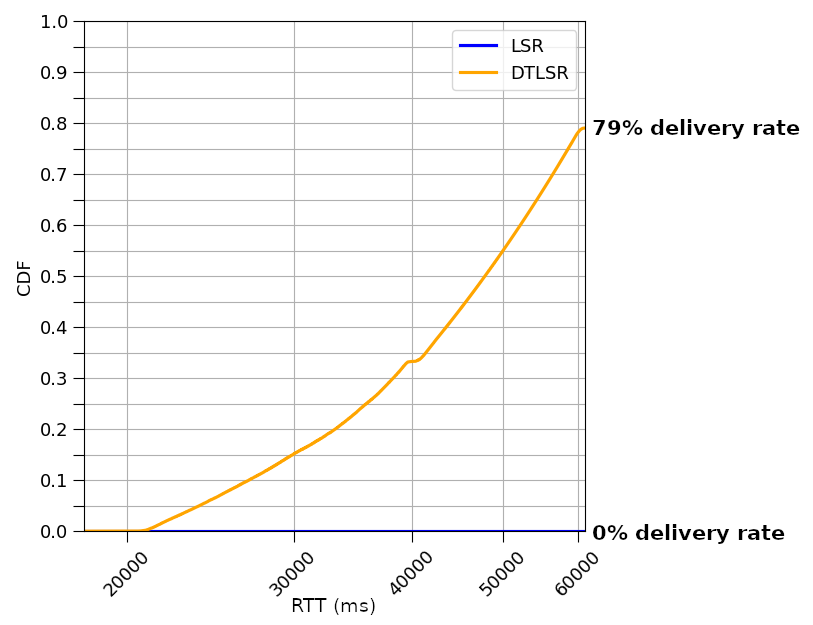
\includegraphics[width=1\linewidth]{delay_full_partition_flap20}
  \caption{Flapping with period $T=\SI{40}{\s}$ (\SI{20}{\s} up, \SI{20}{\s} down).}
  \label{fig:full_partition_flap20}
\end{subfigure}
\caption{}
\label{fig:full_partition_flap}
\end{figure}

We see in Figure~\ref{fig:full_partition_flap} that LSR achieves zero packet delivery, compared to DTLSR achieving upwards of 70\% percent overall. This is notably much more serious than the results above, where LSR achieved a lower but still greater-than-zero delivery, as retransmission-based transport protocols rely on the fact that there is \textit{some} packet delivery, where in the limit of time with retransmissions the probability of delivery approaches 1. However with zero delivery, this limit stays at zero and thus our unreliable network cannot be made reliable with a transport layer protocol. We rely entirely on the routing layer's buffering to achieve any communication whatsoever.

As we increase the flapping period, thus reducing the frequency of boundary events, we again see in Figures~\ref{fig:full_partition_flap5} and \ref{fig:full_partition_flap20} that the packet delivery rate increases. However it is not as large of an increase as seen in the other topologies.

It's interesting to note that we also see an approximately proportional increase in the packet delay as we increase the flapping period, with packets having a delay around four times as large with $T=40$ than $T=10$. This is because packets are spending the vast majority of their time waiting for the link to come back up. It is a similar phenomenon to driving down a long road with traffic lights in series; if the lights are anti-correlated then you will be stopped at each in turn, and your progress down the road will depend almost entirely on the switching frequency of the lights.


\subsection{Box Topology}

Our third topology shown in Figure~\ref{fig:box} is a `box'-shaped one, where we have a low-delay main route and a higher delay backup route when the main one goes down. In this example \texttt{n3-n4} is the main link that we flap, and \texttt{n3-n5-n6-n4} is our higher-delay backup route. The backup link \texttt{n5-n6} has a delay of \SI{10}{\ms}. Thus from \texttt{n1} to \texttt{n2}, our main route has a round-trip delay of \SI{6}{\ms} and our backup route has a round-trip delay of \SI{28}{\ms}.

\begin{minipage}{1\textwidth} \centering
	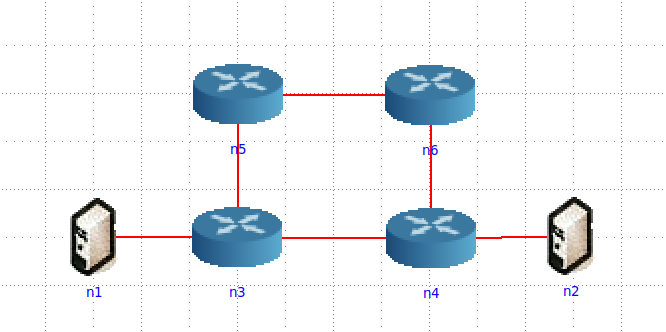
\includegraphics[width=0.6\textwidth]{delay_box_topology}
	\captionof{figure}{`Box' network topology.}
\end{minipage}

%\begin{figure}[H]
%\centering
%\begin{subfigure}{.5\textwidth}
%  \centering
%  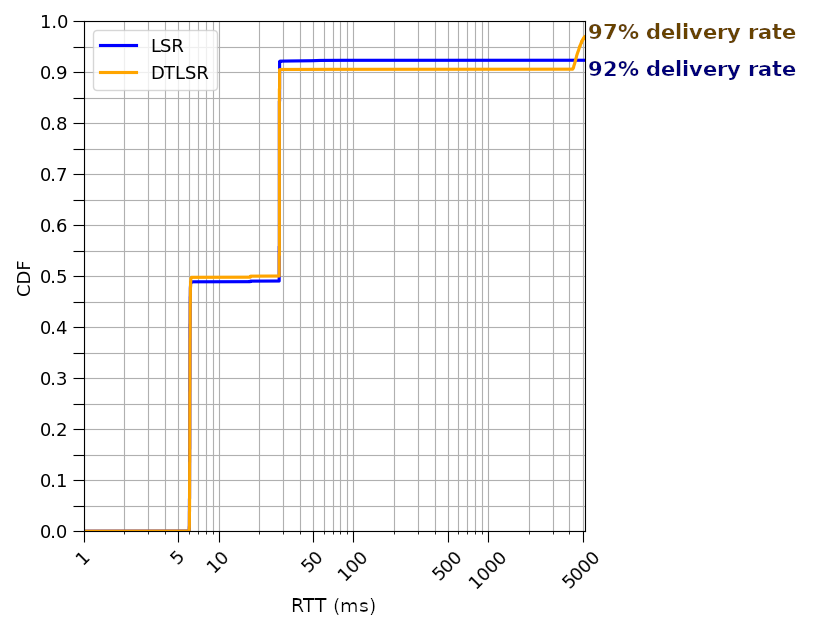
\includegraphics[width=1\linewidth]{delay_box_flap5}
%  \caption{Flapping with period $T=\SI{10}{\s}$ (\SI{5}{\s} up, \SI{5}{\s} down).}
%  \label{fig:box_5}
%\end{subfigure}%
%\begin{subfigure}{.5\textwidth}
%  \centering
%  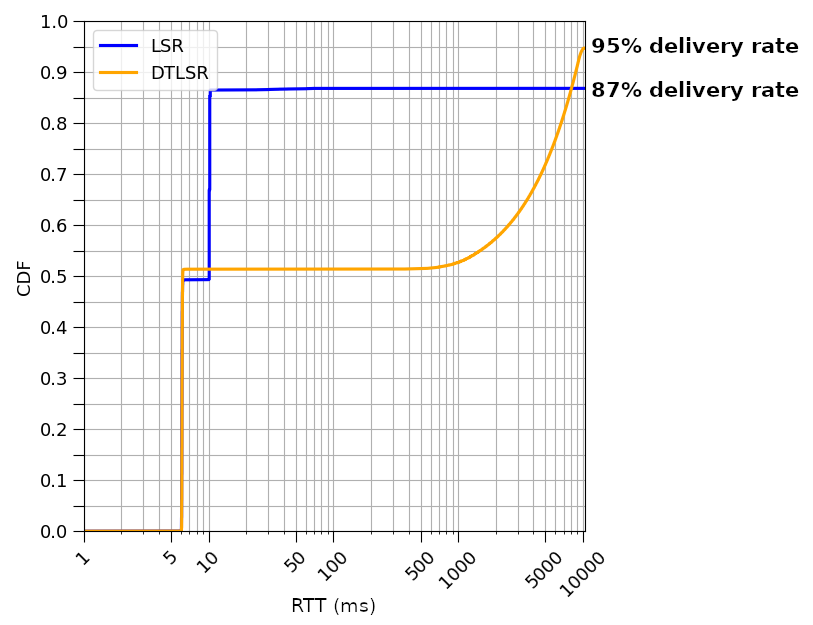
\includegraphics[width=1\linewidth]{delay_box_flap10}
%  \caption{Flapping with period $T=\SI{20}{\s}$ (\SI{10}{\s} up, \SI{10}{\s} down).}
%  \label{fig:box_20}
%\end{subfigure}
%\caption{Cumulative distributions of end-to-end delay between \texttt{n1} and \texttt{n2} under different routing algorithms, while flapping link \texttt{n3-n4}.}
%\label{fig:box}
%\end{figure}

\begin{figure}
\centering
\begin{subfigure}{0.8\textwidth}
  \centering
  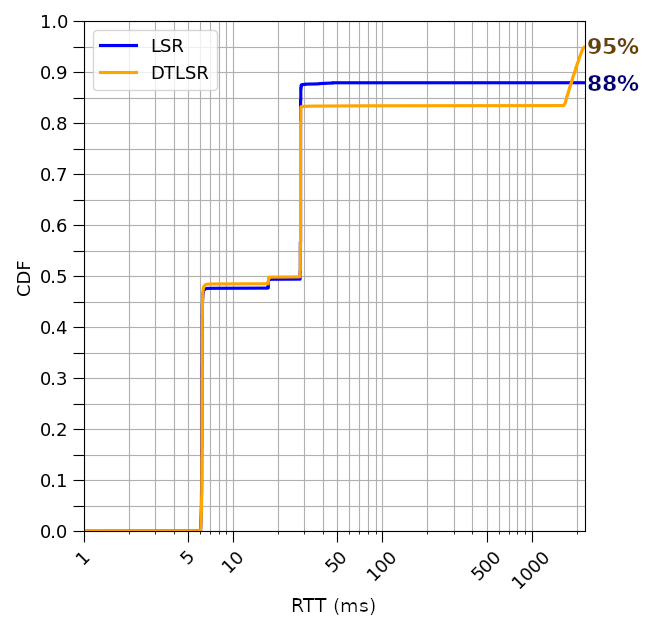
\includegraphics[width=1\linewidth]{delay_box_flap2}
  \caption{Flapping with period $T=\SI{4}{\s}$ (\SI{2}{\s} up, \SI{2}{\s} down).}
  \label{fig:box_20}
\end{subfigure}
\centering
\begin{subfigure}{0.8\textwidth}
  \centering
  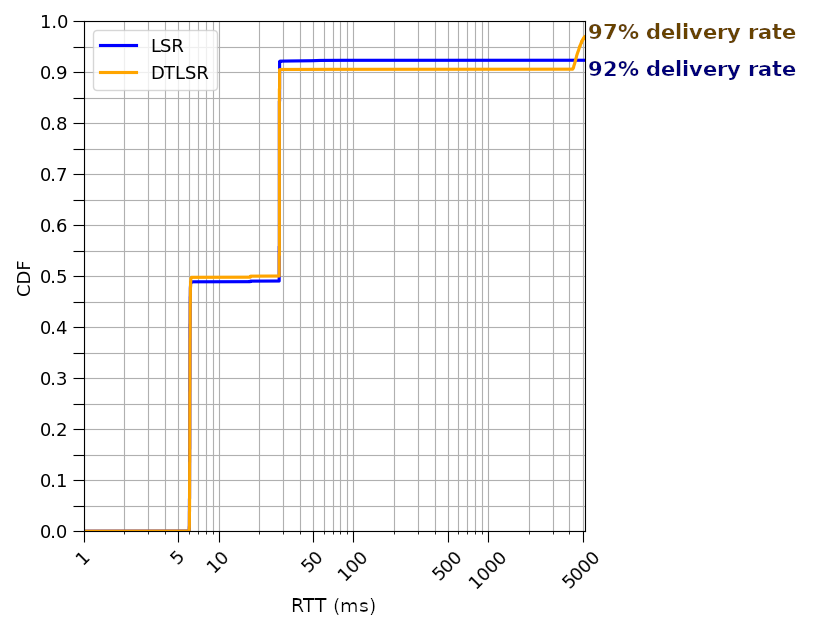
\includegraphics[width=1\linewidth]{delay_box_flap5}
  \caption{Flapping with period $T=\SI{10}{\s}$ (\SI{5}{\s} up, \SI{5}{\s} down).}
  \label{fig:box_5}
\end{subfigure}
\caption{Cumulative distributions of end-to-end delay between \texttt{n1} and \texttt{n2} under different routing algorithms, while flapping link \texttt{n3-n4}.}
\label{fig:box}
\end{figure}

We see in both cases that LSR successfully switches to the backup link whenever the main link goes down, shown by a large proportion of packets having an RTT of approximately \SI{28}{\ms}. As described above, it takes time for the protocol to detect that the link is down and to respond by modifying the routing table, which causes packet losses. Increasing the flapping frequency increases the number of these boundary periods, thus increasing the proportion of time dropping packets. This is reflected in the higher proportion of packets being dropped with a shorter flapping period for LSR.

We again see that DTLSR achieves a higher proportion of delivered packets than LSR. While it is a lot closer than in the partition topology, there is still a marked difference. DTLSR uses its metric to judge the failed link in comparison to the backup link, switching onto it as shown by DTLSR also having a large portion of packets having a delay of around \SI{28}{\ms}. DTLSR is slightly slower to switch the route due to the metrics hysteresis, shown by LSR having a slightly higher proportion of packets with \SI{28}{\ms}. However DTLSR ends up with a higher delivery rate overall due to the packet buffering, shown on the top right of each of the graphs.

As stated above this kind of topology is uncommon in remote and developing regions due to the cost of adding backup links. However it is useful to contrast LSR and DTLSR and show that even with other hardware solutions to failure, DTLSR still has a competitive advantage over LSR in delivery rate.

\section{TCP in Variable-Delay Contexts}

TCP fundamentally does not work well in a variable-delay environment. It works best when the estimated RTT is close to the real delay; in the case where the delay suddenly increases (e.g. a link failure), there will be a long string of packet timeouts in quick succession, dropping the sending window to its minimum size due to the multiplicative decrease (AIMD). Even if these packets have been buffered up before the failure as in DTLSR, the sending node will retransmit them, wasting network resources. TCP will also not transmit any new packets due to the window being constricted, when that is what we actually want to happen due to packets being buffered up by the router. If the failure is longer-term, we may retransmit multiple times, ending up buffering many identical copies of the packet before the link failure. This also has a risk of overflowing the buffer with redundant data. In effect, when the link is down TCP does not transmit new data, nullifying the whole point of the delay-tolerant modifications.

When the network delay has high variability the assumptions made by TCP break down. As a result, we focus on evaluating lossy protocols in the style of UDP.

\section{Summary}

This chapter shows that DTLSR is an effective protocol for improving the delay and packet delivery in an unreliable network environment.

In particular, DTLSR has a strong advantage over LSR in maximising packet delivery in sparsely connected, unreliable networks, especially when link failures cause network partitions. Even when backup links exist, DTLSR is shown to reduce the drop rate of packets by around half compared to LSR. DTLSRs largest advantage is shown in networks with correlated link failures leading to no end-to-end connection, providing a delivery rate upwards of 70\% compared to LSR providing no communication whatsoever.

\chapter{Conclusion}
% JCW -- you need to find some headline figures --- 1/2 numbers that summarise your evaluation --- those can be reapted in the intro, abstract and here. (and obvs also your evaluation.)

\chapter{Bibliography}

\chapter{Appendices}

\chapter{Index}

\chapter{Project Proposal}




%%%%%%%%%%%%%%%%%%%%%%%%%%%%%%%%%%%%%%%%%%%%%%%%%%%%%%%%%%%%%%%%%%%%%%%%%%%%%%%%
%% Index:
%%
\printthesisindex

\end{document}

